
\chapter{液滴模型}

\section{Introduction}

液滴模型（LDM）是历史上第一个被提出来解释原子核不同性质的模型。由于它最近重新引起了人们的兴趣，我们首先简要介绍一下这种唯象模型。我们在本书中讨论该模型的各个方面，并试图从更微观的角度进行解释。在本章中，我们在很大程度上遵循一些经典文本中给出的标准记号，例如：J.
A. Eisenberg 和 W.Greiner \cite{EG70}，A.de Shalit 和 H.Feshbach \cite{SF74}，以及
A.Bohr 和 B.R.Mottelson \cite{BM75}。

将核视为液滴的想法最初来自对其饱和特性的考虑（见下文）以及核具有非常低的可压缩性和明确定义的表面的事实。然而，正如我们将看到的，过于严肃地对待这一观点是误导性的。因为在其他方面，原子核与普通液体没有太多相似之处。例如，液体中两个粒子的平均距离大致由粒子间力达到最小值时给出，对于原子核来说约为$0.7\,\text{fm}$。然而，原子核中的核子平均间隔约为$2.4\,\text{fm}$。这种与普通液体相比巨大差异的一个原因是核子服从费米统计。原子核是一种量子液体，泡利原理会阻止核子彼此靠得太近。因此，散射事件在量子流体中非常稀少，而在普通液体中占主导地位。 

因此，基态（或中等激发态）核内核子的平均自由程的数量级大约和原子核尺度相同，因此，除了统计性质不同外，原子核非常类似于无相互作用的气体。这个事实导致了一些在普通流体的液滴中绝对不存在的结果。例如，在振动的核液滴中（例如，（动态）四极形变）核子的动量分布可能会受到变形的影响；即，它可以是各向异性的，而普通液滴中的速度分布总是各向同性的。量子液滴的这些特性将在第
13 章中更详细地讨论。在这里，相反，我们将遵循LDM思想的历史发展，因为这对于描述原子核的整体性质以及以简单的方式介绍核物理中集体现象的许多概念非常有用。这是第一章的主要目的，我们不会自找麻烦去关注普通液体和量子液体的区别。

\section{半经验公式}

根据上面的讨论，比结合能应当随质量数变化得十分缓慢。事实上，总结合能$B(Z,N)$（其中$N$和$Z$分别是中子和质子的数量）随着核子数量$A$的增加而增长，使得每个核子的结合能$B(N,Z)/A$对于具有超过12个核子的原子核相当的恒定：
\[
\left.\frac{B(N,Z)}{A}\right|_{A>12}\simeq-8.5\,\text{MeV}/\text{nucleon}
\]

比结合能几乎是恒定的这一点是奇怪的。如果有一个$A$粒子的系统，系统中的任意两个粒子相互作用都对结合能有贡献，那么结合能的增长应当大致正比于$\frac{1}{2}A\cdot(A-1)$。于是每粒子结合能应当正比于$A$。事实上，原子中的电子这一系统的结合能就是如此。

核结合能这一迥然不同的性质可以归结于核力的性质：一个原子核中的核子只会和有限几个核子发生相互作用。这源于核力的短程性和Pauli不相容原理和不确定性原理的共同作用。总结合能来源于总动能和总势能行为的细微差异效应；当核子间距离减小时，由于Pauli
原理和不确定性原理，以及核力的硬芯 \cite{Br65a}，动能急剧上升至很大的正值 \cite[p. 252]{BM69}（参见\ref{fig:1_1}），而势能则下降到越来越负的能级。当核子间距足够小（$d\lesssim2\,\text{fm}$）时，动能占主导地位，使得总结合能变为正值；而当距离较大（$d\lesssim3\,\text{fm}$）时，由于核力的短程性，几乎不存在任何势能。最终，在约
$2.4\,\text{fm}$ 处形成一个很浅的极小值，其深度与核力的强度相比是相当微小的。从这些考量中，我们可以清楚地理解为什么在一个核子的相互作用力程范围内只能容纳有限数目的核子。当然，这里我们尚未考虑表面效应和库仑力；我们将在后文中看到，它们必须单独考虑。若暂且忽略这些效应，总结合能就随$A$线性增长。

\begin{figure}[H]
\begin{centering}
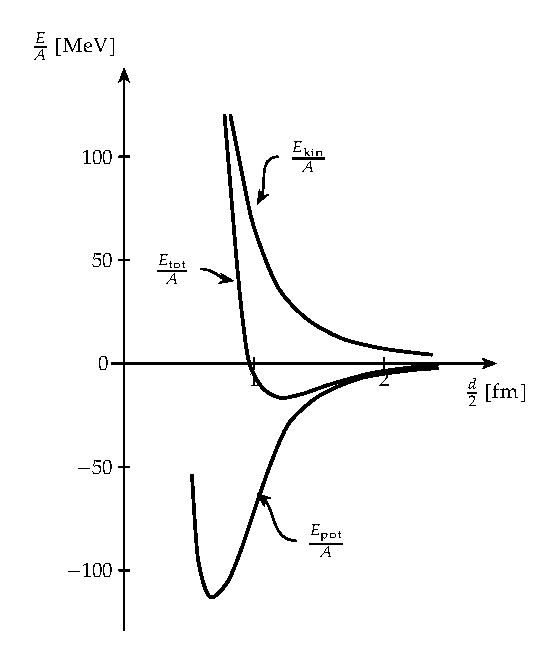
\includegraphics[width=0.45\linewidth]{pictures/1_1}
\par\end{centering}
\centering{}\caption{\label{fig:1_1}核饱和作为动能与势能微小差异效应的定性解释。}
\end{figure}

核力的饱和性质也定性的解释了实验上发现的一些现象（通过电子散射，$\mu$子x-射线等实验发现的），例如原子核内部相对平均的密度和原子核相对确定的表面。现在我们可以用一个具有常数密度和确定表面
\begin{comment}
与模糊的表面相对，实际上就是在说密度分布有一个突变。
\end{comment}
的球来描述原子核了，于是半径为：
\[
R=r_{0}A^{1/3}
\]

经验上讲，参数$r_{0}$的值为：
\[
r_{0}=1.2\,\text{fm}
\]

在\ref{fig:1_2}中，我们可以看出比结合能对于质量数$A$依赖的细节。

\begin{figure}[H]
\begin{centering}
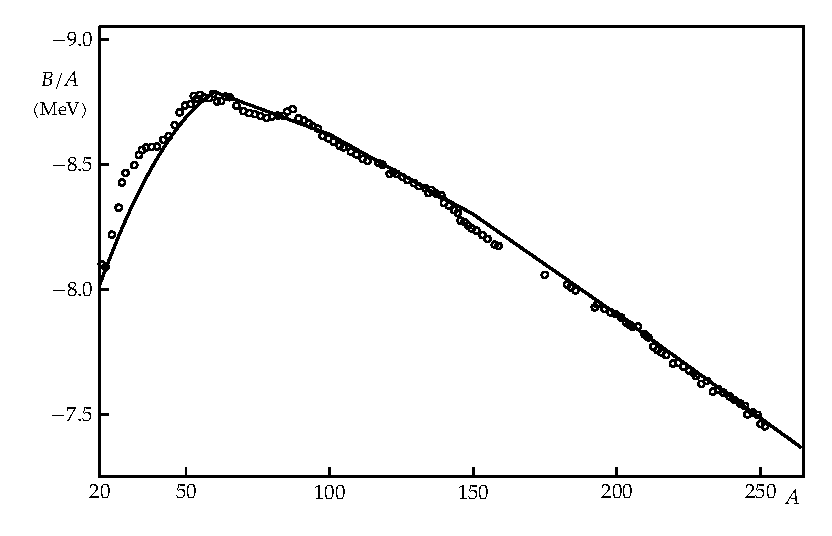
\includegraphics[width=0.68\linewidth]{pictures/1_2}
\par\end{centering}
\centering{}\caption{\label{fig:1_2}实验测得的$\beta$稳定奇$A$核的比结合能和利用类似质量公式计算出的曲线}
\end{figure}

$A=12$以前，比结合能迅速增加直到$B/A\simeq8\,\text{MeV}$，在$A\simeq60$时，比结合能达到最大，稍低于$9\,\text{MeV}$。在此之后，比结合能缓慢下降，直到$A=250$的时候，比结合能降为了大约$7.5\,\text{MeV}$。这是质子的库伦排斥的影响越来越大导致的。

曾经有过很多尝试试图得到$B/A$与$N$、$Z$的函数关系。最著名的公式是Bethe和Weizsci\"acker{[}We
35, BB 36{]}得到的半经验质量公式：
\begin{equation}
B(N,Z)=a_{V}A+a_{S}A^{2/3}+a_{C}\frac{Z^{2}}{A^{1/3}}+a_{I}\frac{(N-Z)^{2}}{A}-\delta(A)\label{eq:semiempirical mass formula}
\end{equation}

拟合得到的合适的参数为{[}MS 66, My 69, MS 69{]}：
\begin{gather*}
a_{V}=-15.68;\quad a_{S}=18.56;\quad a_{C}=0.717;\quad a_{I}=28.1\,\text{MeV}\\
\delta(A)=\begin{cases}
34\cdot A^{-3/4} & \text{偶偶核}\\
0 & \text{奇偶核}\\
-34\cdot A^{-3/4} & \text{奇奇核}
\end{cases}
\end{gather*}

在\ref{fig:1_2}中我们看到，利用这个半经验公式我们得到了非常好的基本符合实验结果的曲线。

接下来我们阐释公式\ref{eq:semiempirical mass formula}的物理意义。第一项通常被称为体积项，因为它正比于$A$，即正比于$R^{3}$。$a_{V}$之所以不等于比结合能$-8.5\,\text{MeV}$，是因为在求比结合能时，需要对很多核做平均，而其它项如$a_{S},a_{C},a_{I}$作平均后是个正的常数。

第二项正比于$A^{2/3}$即$R^{2}$，因此它被称为表面项。它是表面的核子对总结合能的贡献比较小导致的。我们可以从$a_{S}$中得出表面张力系数（定义为单位表面积贡献的能量）：
\[
\sigma=\frac{a_{S}}{4\mathrm{\pi}r^{2}_{0}}=1.03\,\text{MeV\ensuremath{\cdot}\text{fm}}^{-2}
\]

第三项考虑了库伦相互作用。如果我们近似的把原子核看成是电荷均匀分布的球体，那么它就可以计算出来。原子核体系的库仑能正比于质子数的平方，反比于半径。

因为质子会互相排斥，似乎原子核会倾向于有更多的中子，但这是并未考虑泡利不相容原理的结果。事实上，如果一个质子发生$\beta$衰变变成中子，这个中子会成为中子费米面之上的态（见第二章），这从能量的角度上讲是不容易发生的。第四项即考虑了这一平衡，根据费米气体模型，它正比于$(N-Z)^{2}/A$，它会促使质子数和中子数相同，被称为对称能。这一结合能和$N-Z$的二次方关系和实验也符合的非常好。

考虑了这四项之后，和实验结果唯一的不同就是考虑偶偶核，奇偶核和奇奇核时的区别。在第六章我们会看到，这是所谓的对效应导致的。我们在第五项中考虑了这一点。

第十三章我们讨论Thomas-Fermi方法时会再次讨论半经验质量公式。

需要指出的是，半经验质量公式只是整体上很好的拟合了结合能关于$A$的函数，局部上仍会出现较大的偏离。这主要是壳效应导致的，我们在2.9部分会讨论这一点。

\section{形变参数}

到目前为止，我们只研究了液滴模型的静态性质。接下来我们会假设原子核具有一个确定的表面，但却不一定是球面。并且我们会想象它发生动力学形变和表面的振动。

在我们研究这些振动之前，我们必须用一些参数来描述表面。一个可能的方式是用原子核中心到表面的径矢长度来描述：
\begin{equation}
R=R(\theta,\phi)=R_{0}\left(1+\alpha_{00}+\sum^{\infty}_{\lambda=1}\sum^{\lambda}_{\mu=-\lambda}\alpha^{*}_{\lambda\mu}Y_{\lambda\mu}(\theta,\phi)\right)\label{eq:expansion of R}
\end{equation}

这里$R_{0}$是具有相同体积的球面的半径
\begin{comment}
这里的所有$\alpha$都是小参数。
\end{comment}
。这样的表面不是最一般的形式\footnote{例如裂变中裂成两半的核。}，但却是在核结构中非常有用的形式。

参数$\alpha_{00}$描述了核的体积变化。我们知道原子核的不可压缩性非常之强，因此在发生任何形变时，核的体积应当保持不变：
\[
V=\frac{4}{3}\mathrm{\pi}R^{3}_{0}
\]

这定义了参数$\alpha_{00}$，至多到二阶，我们得到\cite{EG70}：
\[
\alpha_{00}=-\frac{1}{4\mathrm{\pi}}\sum_{\lambda\geq1,\mu}\left|\alpha_{\lambda\mu}\right|^{2}
\]

\begin{booknote*}
使用$R(\theta,\phi)$计算核的体积，应当有：
\begin{align*}
V & =\int^{R}_{0}r^{2}\sin\theta\mathrm{d}r\mathrm{d}\theta\mathrm{d}\phi=\frac{1}{3}\int R^{3}\sin\theta\mathrm{d}\theta\mathrm{d}\phi\\
 & =\frac{1}{3}R^{3}_{0}\int\left(1+\alpha_{00}+\sum^{\infty}_{\lambda=1}\sum^{\lambda}_{\mu=-\lambda}\alpha^{*}_{\lambda\mu}Y_{\lambda\mu}(\theta,\phi)\right)^{3}\sin\theta\mathrm{d}\theta\mathrm{d}\phi
\end{align*}

保留到$\alpha$的二阶项，得到：
\begin{align*}
V & =\frac{1}{3}R^{3}_{0}\int1+3\alpha_{00}+3\alpha^{2}_{00}+3(1+2\alpha_{0})\left(\sum^{\infty}_{\lambda=1}\sum^{\lambda}_{\mu=-\lambda}\alpha^{*}_{\lambda\mu}Y_{\lambda\mu}(\theta,\phi)\right)\\
 & +3\left(\sum^{\infty}_{\lambda=1}\sum^{\lambda}_{\mu=-\lambda}\alpha^{*}_{\lambda\mu}Y_{\lambda\mu}(\theta,\phi)\right)^{2}\sin\theta\mathrm{d}\theta\mathrm{d}\phi
\end{align*}

球谐函数的一次项积分应当为零，二次项可以如下得到：由于$R$为实数，因此$R^{2}$可以写为$R^{*}R$，由此可以利用球谐函数的正交性得到结果：
\[
V=\frac{4}{3}\mathrm{\pi}R^{3}_{0}+4\mathrm{\pi}\alpha_{00}(1+\alpha_{00})R^{3}_{0}+\sum_{\lambda\geq1,\mu}\left|\alpha_{\lambda\mu}\right|^{2}R^{3}_{0}
\]

由此我们得到：
\[
4\mathrm{\pi}\alpha_{00}(1+\alpha_{00})R^{3}_{0}+\sum_{\lambda\geq1,\mu}\left|\alpha_{\lambda\mu}\right|^{2}R^{3}_{0}=0
\]
我们考虑如下方程：
\[
x(1+x)+a=0
\]

其中$x$，$a$均是小量，我们可以解得：
\begin{align*}
x=\frac{-1\pm\sqrt{1-4a}}{2}
\end{align*}

保留到一阶，得：
\[
x=-\frac{1}{2}\pm\frac{1}{2}(1-2a)=-a/(a-1)
\]

由于$x$是小量，因此$x=-a$。

回归到上述问题，我们得到：
\[
\alpha_{00}=-\frac{1}{4\mathrm{\pi}}\sum_{\lambda\geq1,\mu}\left|\alpha_{\lambda\mu}\right|^{2}
\]
\end{booknote*}
$\lambda=1$的项主要描述了整个体系的平移（至少对于小形变来说）。当原点取在质心处时，$\alpha_{1\mu}$这三个参数可以唯一确定。此时有：
\[
\int_{V}\boldsymbol{r}\,\mathrm{d}^{3}\boldsymbol{r}=0
\]

\begin{booknote*}
考虑质心发生了移动，$(x,y,z)$变成了$(x+x_{0},y+y_{0},z+z_{0})$，其中$x_{0},y_{0},z_{0}$均为小量。把直角坐标转换成球坐标，保留到一阶得到：
\[
R^{\prime}=\sqrt{(x+x_{0})^{2}+(y+y_{0})^{2}+(z+z_{0})^{2}}\approx R+\frac{xx_{0}+yy_{0}+zz_{0}}{x^{2}+y^{2}+z^{2}}
\]

因此把$R^{\prime}$用$\theta^{\prime},\phi^{\prime}$表示出来，必定有：
\[
R^{\prime}=R+\sin\theta^{\prime}\cos\phi^{\prime}x_{0}+\sin\theta^{\prime}\sin\phi^{\prime}y_{0}+\cos\theta^{\prime}z_{0}
\]

根据球谐函数的表达式，一阶项可以写成$Y_{1,-1}$，$Y_{1,0}$，$Y_{1,1}$的线性和。

我们由此证明了$\lambda=1$的项描述了整个体系的平移。
\end{booknote*}
如果展开式\ref{eq:expansion of R}仅包含$\lambda$的偶数值，则该条件自动满足
\begin{comment}
我不知道他为什么要强调这一点。
\end{comment}
。在其他情形下，$\alpha_{1\mu}$则从$\alpha_{\lambda\mu}\,(\lambda>2)$的二阶项开始
\begin{comment}
我看不懂它在说什么。
\end{comment}
。因此，由于我们在后续讨论中将限制于小形变情形，我们将同时略去$\alpha_{00}$与$\alpha_{1\mu}$
\begin{comment}
为什么可以忽略$\alpha_{00}$？我认为是不能省的，因此后面的推导没有省略，并且得到了正确的结果。
\end{comment}
。

看一看展开式\ref{eq:expansion of R}中最低阶的多级形变是有益的，如\ref{fig:1_3}。$\lambda=2$的对应的形变看起来像椭球形变。然而，需要注意的是这仅仅精确到了小参数的一阶。一个真正的椭球的表达式中，$\lambda>2$的项也都是存在的。

\begin{figure}[H]
\begin{centering}
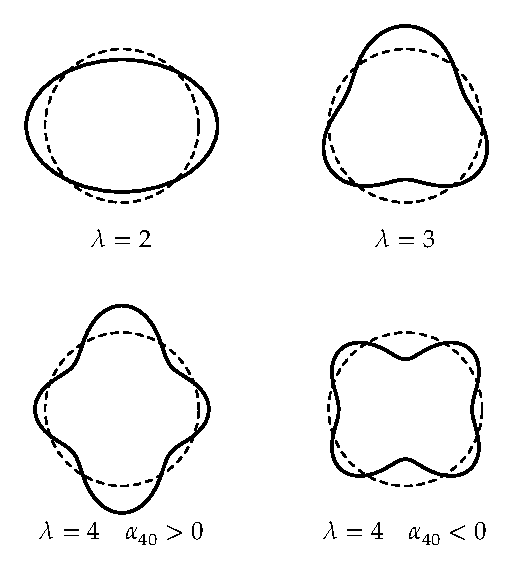
\includegraphics[width=0.48\linewidth]{pictures/1_3}
\par\end{centering}
\centering{}\caption{\label{fig:1_3}多级形变}
\end{figure}

此外，径矢长度$R$在反演变换和转动变换下应当是不变的
\begin{comment}
形式应当是不变的，变化的只是参数的值。根据球谐函数的完备性，我觉得这并不构成所谓的“限制”，只是我们推导出了坐标系在相应变换下新参数和旧参数的关系。
\end{comment}
，这对$\alpha_{\lambda\mu}$构成了限制。为此，$\alpha_{\lambda\mu}$在反演变换下必须乘上$(-)^{\lambda}$，并且在转动变换下必须像一个球谐函数一样变换。即如果转动了Euler角$\Omega=(\alpha,\beta,\gamma)$的话，应当有：
\begin{align*}
(Y_{\lambda\mu})_{\text{new}} & =\sum_{\mu^{\prime}}D^{\lambda}_{\mu^{\prime}\mu}(\Omega)(Y_{\lambda\mu^{\prime}})_{\text{old}}\\
a_{\lambda\mu} & =\sum_{\mu^{\prime}}D^{\lambda}_{\mu^{\prime}\mu}(\Omega)\alpha_{\lambda\mu^{\prime}}
\end{align*}

这里$D^{\lambda}_{\mu^{\prime}\mu}(\Omega)$是转动的Wigner函数，$a_{\lambda\mu}$是转动后参考系中的形变参数。
\begin{booknote*}
变换参考系后的径矢长度$R^{\prime}$用新参考系中的坐标$\theta^{\prime}$，$\phi^{\prime}$表示为：
\[
R^{\prime}(\theta^{\prime},\phi^{\prime})=R_{0}\left(1+\alpha_{00}+\sum^{\infty}_{\lambda=2}\sum_{\mu}a^{*}_{\lambda\mu}Y_{\lambda\mu}(\theta^{\prime},\phi^{\prime})\right)
\]

利用：
\[
Y_{\lambda\mu}(\theta^{\prime},\phi^{\prime})=\sum_{\mu^{\prime}}D^{\lambda}_{\mu^{\prime}\mu}(\Omega)Y_{\lambda\mu^{\prime}}(\theta,\phi)
\]

得到：
\[
R^{\prime}(\theta^{\prime},\phi^{\prime})=R_{0}\left(1+\alpha_{00}+\sum^{\infty}_{\lambda=2}\sum_{\mu\mu^{\prime}}a^{*}_{\lambda\mu}D^{\lambda}_{\mu^{\prime}\mu}(\Omega)Y_{\lambda\mu^{\prime}}(\theta,\phi)\right)
\]

因此要求：
\[
\sum_{\mu}a^{*}_{\lambda\mu}D^{\lambda}_{\mu^{\prime}\mu}(\Omega)=\alpha^{*}_{\lambda\mu^{\prime}}
\]

利用$D^{\lambda}_{\mu^{\prime}\mu}(\Omega)=D^{\lambda*}_{\mu\mu^{\prime}}(\Omega^{-1})$，得到：
\[
\sum_{\mu}a_{\lambda\mu}D^{\lambda}_{\mu\mu^{\prime}}(\Omega^{-1})=\alpha_{\lambda\mu^{\prime}}
\]

此即：
\[
a_{\lambda\mu}=\sum_{\mu^{\prime}}D^{\lambda}_{\mu^{\prime}\mu}(\Omega)\alpha_{\lambda\mu^{\prime}}
\]

由此得到：
\[
R^{\prime}(\theta^{\prime},\phi^{\prime})=R_{0}\left(1+\alpha_{00}+\sum^{\infty}_{\lambda=2}\sum_{\mu^{\prime}}\alpha^{*}_{\lambda\mu^{\prime}}Y_{\lambda\mu^{\prime}}(\theta,\phi)\right)=R(\theta,\phi)
\]

由推导中也看出了一开始引入的$\alpha^{*}$中star的作用。
\end{booknote*}
为了确保\ref{eq:expansion of R}中的径矢长度$R$是实的，我们必须利用性质$Y^{*}_{\lambda\mu}=(-)^{\mu}Y_{\lambda,-\mu}$得到：
\[
\alpha^{*}_{\lambda\mu}=(-)^{\mu}\alpha_{\lambda,-\mu}
\]

之后可以证明，这恰恰是$\alpha_{\lambda\mu}$在时间反演下的行为。
\begin{booknote*}
利用上述性质，应当有：
\begin{align*}
\alpha^{*}_{\lambda\mu}Y_{\lambda\mu}+\alpha^{*}_{\lambda,-\mu}Y_{\lambda,-\mu} & =\alpha^{*}_{\lambda\mu}Y_{\lambda\mu}+\alpha^{*}_{\lambda,-\mu}(-)^{\mu}Y^{*}_{\lambda\mu}
\end{align*}

为了使它们组合出常数，两项应当互为共轭，得到：
\[
\alpha^{*}_{\lambda\mu}=(-)^{\mu}\alpha_{\lambda,-\mu}
\]
\end{booknote*}
在讨论普适的表面多级振动之前，我们需要提及两种特殊的情况：
\begin{enumerate}
\item 第一种是轴对称的形变。如果选取$z$轴为对称轴，我们会发现$\alpha_{\lambda\mu}$只有$\mu=0$的情况下才不为零。$\alpha_{\lambda0}$通常称作$\beta_{\lambda}$。
\item 在偶极形变（$\lambda=2$）的情况下，我们有五个$\alpha_{\lambda\mu}$参数。它们并没有都描述了液滴的形状。事实上，其中有三个描述了液滴的取向，和三个Euler角有关。通过一个合适的转动，我们可以把参考系转动到三个轴1，2，3表征的体坐标系，这三个轴和液滴的质量分布的主轴是对应的。转动之后，五个参数$\alpha_{2\mu}$变为了两个独立变量$a_{20}$和$a_{22}=a_{2,-2}$（$a_{21}=a_{2,-1}=0$），这两个变量和三个Euler角一起，完整的描述了这个系统。为了方便，我们引入Hill-Wheeler坐标$\beta,\gamma$，他们和$a_{20}$，$a_{22}$的关系为：
\begin{align*}
a_{20} & =\beta\cdot\cos\gamma\\
a_{22} & =\frac{1}{\sqrt{2}}\cdot\beta\cdot\sin\gamma
\end{align*}

由此我们得到：
\[
\sum_{\mu}\left|\alpha_{2\mu}\right|^{2}=a^{2}_{20}+2a^{2}_{22}=\beta^{2}
\]

以及：
\[
R(\theta,\phi)=R_{0}\left\{ 1+\beta\sqrt{\frac{5}{16\mathrm{\pi}}}[\cos\gamma(3\cos^{2}\theta-1)+\sqrt{3}\sin\gamma\sin^{2}\theta\cos2\phi]\right\} 
\]

\end{enumerate}
在\ref{fig:1_4}中，我们在极坐标$\beta$，$\gamma$中表示了偶极形变的形状。我们可以看出：
\begin{enumerate}
\item $\gamma$的值为$0^{\circ}$，$120^{\circ}$，$240^{\circ}$时，为以3，1，2轴为对称轴的长椭球。
\item $\gamma$的值为$180^{\circ}$，$300^{\circ}$，$60^{\circ}$时为对应的扁椭球。
\item 其他情形对应三轴形变（triaxial shapes）
\begin{comment}
按照我画的图看，意思应该是不是柱对称的。
\end{comment}
。
\item 存在离散对称性，也就是说，我们可以随意交换三个轴而不改变形状。这意味着点群$D_{2}$下的不变性
\begin{comment}
提这个有意义吗？——看到点群就烦的译者。
\end{comment}
。因此，$0<\gamma<60^{\circ}$可以描述所有偶极形变，其它形状可以通过交换轴得到。
\end{enumerate}
\begin{figure}[H]
\begin{centering}
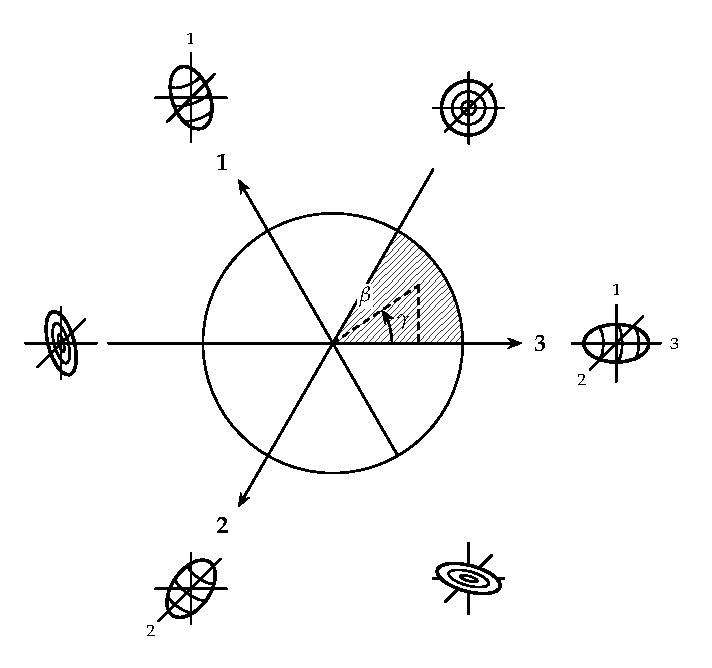
\includegraphics[width=0.52\linewidth]{pictures/1_4}
\par\end{centering}
\centering{}\caption{\label{fig:1_4}Hill-Wheeler坐标下的原子核形状}
\end{figure}

\begin{enumerate}
\item 可以计算出$\beta$和$\gamma$引起的椭球半轴变化量：
\begin{align*}
\delta R_{1} & =R(\frac{\mathrm{\pi}}{2},0)-R_{0}=R_{0}\sqrt{\frac{5}{4\mathrm{\pi}}}\beta\cos\left(\gamma-\frac{2\mathrm{\pi}}{3}\right)\\
\delta R_{2} & =R(\frac{\mathrm{\pi}}{2},\frac{\mathrm{\pi}}{2})-R_{0}=R_{0}\sqrt{\frac{5}{4\mathrm{\pi}}}\beta\cos\left(\gamma+\frac{2\mathrm{\pi}}{3}\right)\\
\delta R_{3} & =R(0,0)-R_{0}=R_{0}\sqrt{\frac{5}{4\mathrm{\pi}}}\beta\cos\gamma
\end{align*}

即：
\[
\delta R_{\kappa}=R_{0}\sqrt{\frac{5}{4\mathrm{\pi}}}\beta\cos\left(\gamma-\frac{2\mathrm{\pi}}{3}\kappa\right),\quad\kappa=1,2,3
\]

我们必须强调，$\beta$和$\gamma$仅在小参数的情况下描述了椭球形变。
\end{enumerate}

\section{球形的表面振动}

第一种类型的激发是动力学的形状或表面振动。此时的动力学变量是描述表面的参数，例如\ref{eq:expansion of R}中的$\alpha_{\lambda\mu}(\lambda\geq2)$。它们被认为是时间的函数：$\alpha_{\lambda\mu}(t)$。我们可以期待，低能激发实际上是$\alpha_{\lambda\mu}=0$（对应球面）附近的一些小振动，描述这一过程的Hamilton量具有谐振子的形式：
\begin{equation}
H_{\text{coll}}=T+V=\frac{1}{2}\sum_{\lambda\mu}\left(B_{\lambda}\left|\dot{\alpha}_{\lambda\mu}\right|^{2}+C_{\lambda}\left|\alpha_{\lambda\mu}\right|^{2}\right)\label{eq:Hamiltonian of vibrating sphere}
\end{equation}

这里惯性系数$B_{\lambda}$和刚度系数$C_{\lambda}$是实参数。这实际上是由转动不变和时间反演不变\footnote{关于时间反演，Messiah\cite{Me61}中有更多细节。在无自旋系统中，同这里一样，时间反演与复共轭相联系。}所确定的唯一可能的二次形式。

利用正则量子化，我们得到量子化后的形式：
\[
\hat{H}_{\text{coll}}=\sum_{\lambda\mu}\hbar\Omega_{\lambda}\left(B^{\dagger}_{\lambda\mu}B_{\lambda\mu}+\frac{1}{2}\right)
\]

这里频率为：
\[
\Omega_{\lambda}=\left(\frac{C_{\lambda}}{B_{\lambda}}\right)^{\frac{1}{2}}
\]

算符$B_{\lambda\mu}$满足Bose对易关系：
\[
[B_{\lambda\mu},B_{\lambda^{\prime}\mu^{\prime}}]=0;\quad[B_{\lambda\mu},B^{\dagger}_{\lambda^{\prime}\mu^{\prime}}]=\delta_{\lambda\lambda^{\prime}}\delta_{\mu\mu^{\prime}}
\]

并且存在一个Bose真空$|0\rangle$使得$B_{\lambda\mu}|0\rangle=0$。Bose算符$B_{\lambda\mu}$和坐标算符$\hat{\alpha}_{\lambda\mu}$和相应的动量算符$\hat{\pi}_{\lambda\mu}$的关系如下：
\begin{align*}
\hat{\alpha}_{\lambda\mu} & =\left(\frac{\hbar}{2B_{\lambda}\Omega_{\lambda}}\right)^{\frac{1}{2}}[B^{\dagger}_{\lambda\mu}+(-)^{\mu}B_{\lambda,-\mu}]\\
\hat{\pi}_{\lambda\mu} & =\mathrm{i}\left(\frac{\hbar}{2}B_{\lambda}\Omega_{\lambda}\right)^{\frac{1}{2}}[(-)^{\mu}B^{\dagger}_{\lambda,-\mu}-B_{\lambda\mu}]
\end{align*}

\begin{booknote*}
根据Hamilton量写出动量：
\begin{align*}
\pi_{\lambda\mu} & =\frac{\partial H_{\text{coll}}}{\partial\dot{\alpha}_{\lambda\mu}}=\frac{1}{2}\sum_{\lambda^{\prime}\mu^{\prime}}B_{\lambda^{\prime}}\frac{\partial}{\partial\dot{\alpha}_{\lambda\mu}}\dot{\alpha}^{*}_{\lambda^{\prime}\mu^{\prime}}\dot{\alpha}_{\lambda^{\prime}\mu^{\prime}}\\
 & =\frac{1}{2}\sum_{\lambda^{\prime}\mu^{\prime}}B_{\lambda^{\prime}}\frac{\partial}{\partial\dot{\alpha}_{\lambda\mu}}(-)^{\mu^{\prime}}\dot{\alpha}_{\lambda^{\prime},-\mu^{\prime}}\dot{\alpha}_{\lambda^{\prime}\mu^{\prime}}\\
 & =B_{\lambda}\dot{\alpha}^{*}_{\lambda\mu}
\end{align*}

于是Hamilton量变为：
\[
H_{\text{coll}}=\frac{1}{2}\sum_{\lambda\mu}\left(\frac{1}{B_{\lambda}}\left|\pi_{\lambda\mu}\right|^{2}+C_{\lambda}\left|\alpha_{\lambda\mu}\right|^{2}\right)
\]

根据正则量子化步骤，引入Bose对易关系：
\[
[\hat{\alpha}_{\lambda\mu},\hat{\pi}_{\lambda^{\prime}\mu^{\prime}}]=\mathrm{i}\hbar\delta_{\lambda\lambda^{\prime}}\delta_{\mu\mu^{\prime}}
\]

并按照前面的定义引入$B_{\lambda\mu}$和$B^{\dagger}_{\lambda\mu}$，经验证可以满足产生湮灭算符的对应关系。与此同时，Hamilton量变为期望的谐振子形式。
\end{booknote*}
从上面的讨论中，我们得到对每一个$\lambda$，都有一个相应的表面振动谐振子谱与之对应，正如\ref{fig:1_5}。

\begin{figure}[H]
\begin{centering}
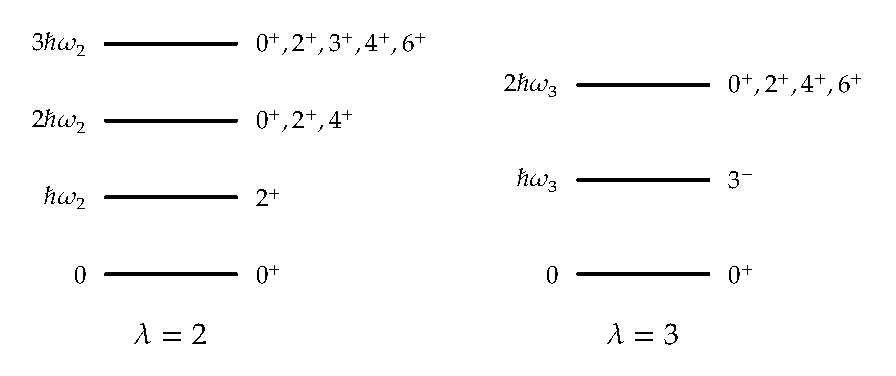
\includegraphics[width=0.55\linewidth]{pictures/1_5}
\par\end{centering}
\centering{}\caption{\label{fig:1_5}四极（$\lambda=2$）和八极（$\lambda=3$）表面振动的简谐能谱}
\end{figure}

根据$\alpha_{\lambda\mu}$和$B^{\dagger}_{\lambda\mu}$在坐标系转动下都如同球张量一样变换，我们可以得到$B^{\dagger}_{\lambda\mu}$与角动量算符的对易关系，并发现单玻色子态$|\lambda\mu\rangle=B^{\dagger}_{\lambda\mu}|0\rangle$有角动量$I=\lambda$，$z$-分量$M=\mu$，宇称$(-)^{\lambda}$。
\begin{booknote*}
坐标变换下：
\[
\hat{a}_{\lambda\mu}=\sum_{\mu^{\prime}}D^{\lambda}_{\mu^{\prime}\mu}(\Omega)\hat{\alpha}_{\lambda\mu^{\prime}}
\]

由此$\hat{\pi}_{\lambda\mu}$在坐标变换下：
\begin{align*}
\hat{p}_{\lambda\mu} & =B_{\lambda}\dot{\hat{\alpha}}^{*}_{\lambda\mu}=B_{\lambda}\sum_{\mu^{\prime}}D^{\lambda*}_{\mu^{\prime}\mu}(\Omega)\dot{\hat{\alpha}}^{*}_{\lambda\mu^{\prime}}\\
 & =\sum_{\mu^{\prime}}D^{\lambda*}_{\mu^{\prime}\mu}(\Omega)\hat{\pi}_{\lambda\mu^{\prime}}
\end{align*}

可知$\hat{p}^{\dagger}_{\lambda\mu}=\sum_{\mu^{\prime}}D^{\lambda}_{\mu^{\prime}\mu}(\Omega)\hat{\mathrm{\pi}}_{\lambda\mu^{\prime}}$，与$\hat{\alpha}_{\lambda\mu}$的变换相同。再根据：
\[
B^{\dagger}_{\lambda\mu}=\frac{1}{2}\left[\left(\frac{2}{\hbar}B_{\lambda}\Omega_{\lambda}\right)^{\frac{1}{2}}\hat{\alpha}_{\lambda\mu}+\mathrm{i}\left(\frac{2}{\hbar B_{\lambda}\Omega_{\lambda}}\right)^{\frac{1}{2}}\hat{\mathrm{\pi}}^{\dagger}_{\lambda\mu}\right]
\]

可知$B^{\dagger}_{\lambda\mu}$同$\alpha_{\lambda\mu}$变换也相同。之后的结论参考角动量与球张量。
\end{booknote*}
为了构建多玻色子态，我们必须利用角动量耦合的规则，并且考虑置换对称性
\begin{comment}
为何要考虑？
\end{comment}
。例如，考虑两个四极玻色子（$\lambda=2$）的叠加，三种可能的组合为$I^{\pi}=0^{+},2^{+},4^{+}$。
\[
|IM\rangle=\frac{1}{\sqrt{2}}\sum_{\mu_{1}\mu_{2}}C^{22I}_{\mu_{1}\mu_{2}M}B^{\dagger}_{2\mu_{1}}B^{\dagger}_{2\mu_{2}}|0\rangle
\]

$I=1,3$的态都会消失，因为Clebsch-Gordon系数\footnote{这里我们利用$C^{j_{1}j_{2}j_{3}}_{m_{1}m_{2}m_{3}}$来表示$\langle j_{1}m_{1}j_{2}m_{2}|j_{1}j_{2}j_{3}m_{2}\rangle$。}的在$\mu_{1}$和$\mu_{2}$交换时的性质：
\[
C^{22I}_{\mu_{1}\mu_{2}M}=(-)^{I}C^{22I}_{\mu_{2}\mu_{1}M}
\]

事实上，许多球形核的谱中有一个低能的$2^{+}$态。大约在两倍的激发能
\begin{comment}
第一激发态的能量。
\end{comment}
处，还有所谓的两玻色子三重态（$0^{+}$，$2^{+}$，$4^{+}$），然而，这三个态的能谱通常分开一点点。

常数$B_{\lambda}$和$C_{\lambda}$可以在流体图像中计算出来；它们取决于与表面振动相关的流动。因此，有必要假设液滴内流体运动的性质。
\begin{comment}
此时，我们需要再次讨论核液体这一概念的含义。在第十三章，我们将会仔细研究这一点并且发现核实际上是费米液体而不是普通的液体，这一点非常重要。（我觉得这是不需要说的话，但是是书上有的，我把它放在了脚注里。
\end{comment}
我们可以做的最简单的假设是流体是无旋的，即$\nabla\times\boldsymbol{v}(\boldsymbol{r})=0$，这里$\boldsymbol{v}$是速度场。我们在第十三章中还会研究这一假定，但是现在先让我们接受它：
\[
\boldsymbol{v}(t)=-\nabla\Phi(\boldsymbol{r})
\]

下一个假设是不可压缩性，这对于原子核来说是十分合理的。这意味着原子核密度是个常数（$\dot{\rho}=0$），根据连续性方程，我们可以得到：
\[
\nabla\cdot\boldsymbol{v}=0
\]

由此，得到：
\[
\nabla^{2}\Phi=0
\]

上述方程在原点处不发散的最一般的解是：
\[
\Phi(\boldsymbol{r})=\sum_{\lambda\mu}d^{*}_{\lambda\mu}r^{\lambda}Y_{\lambda\mu}(\theta,\phi)
\]

对于小形变，精确到一阶，边界条件可以为：
\[
v_{r}=-\frac{\partial}{\partial r}\Phi=\dot{R}\quad\text{at}\quad r=R_{0}
\]

由此，代入\ref{eq:expansion of R}即可得到系数$d_{\lambda\mu}$和$\alpha_{\lambda\mu}$的关系：
\[
d_{\lambda\mu}=-\frac{1}{\lambda}R^{2-\lambda}_{0}\dot{\alpha}_{\lambda\mu}
\]

\begin{booknote*}
边界条件为：
\[
-\sum_{\lambda\mu}d^{*}_{\lambda\mu}\lambda R^{\lambda-1}_{0}Y_{\lambda\mu}(\theta,\phi)=R_{0}\left(\sum_{\lambda\mu}\dot{\alpha}^{*}_{\lambda\mu}Y_{\lambda\mu}(\theta,\phi)\right)
\]

根据球谐函数正交性可得：
\[
d^{*}_{\lambda\mu}=-\frac{1}{\lambda}R^{2-\lambda}_{0}\dot{\alpha}^{*}_{\lambda\mu}
\]
\end{booknote*}
表面振动的动能为：
\[
T=\frac{m}{2}\rho\int_{V}v^{2}(\boldsymbol{r})\,\mathrm{d}^{3}\boldsymbol{r}=\frac{m}{2}\rho\int_{V}\left|\nabla\Phi\right|^{2}\,\mathrm{d}^{3}\boldsymbol{r}=\frac{m}{2}\rho\oint_{S}\Phi^{*}\nabla\Phi\cdot\mathrm{d}\boldsymbol{S}
\]

这里$\rho$是质量为$m$的核子密度，是一个常数。利用球谐函数的梯度公式
\begin{comment}
狗屁，哪里用到了。
\end{comment}
，我们得到小形变近似下的动能为：
\begin{equation}
T=\frac{R^{5}_{0}m\rho}{2}\sum_{\lambda\mu}\frac{\left|\dot{\alpha}_{\lambda\mu}\right|^{2}}{\lambda}\label{eq:kinetic energy of little alpha}
\end{equation}

\begin{booknote*}
利由于梯度要与$\mathrm{d}\boldsymbol{S}$相乘，因此只需要计算$r$分量，用球坐标梯度公式得：
\begin{align*}
\nabla r^{\lambda}Y_{\lambda\mu}(\theta,\phi) & =\lambda r^{\lambda-1}Y_{\lambda\mu}(\theta,\phi)\hat{\boldsymbol{e}}_{r}
\end{align*}

由此推得动能为：
\begin{align*}
T & =\frac{m\rho}{2}\oint_{S}\sum_{\lambda\mu}d_{\lambda\mu}r^{\lambda}Y^{*}_{\lambda\mu}(\theta,\phi)\nabla\left(\sum_{\lambda^{\prime}\mu^{\prime}}d^{*}_{\lambda^{\prime}\mu^{\prime}}r^{\lambda^{\prime}}Y_{\lambda^{\prime}\mu^{\prime}}(\theta,\phi)\right)\cdot\mathrm{d}\boldsymbol{S}\\
 & =\frac{m\rho}{2}\sum_{\lambda\mu}\sum_{\lambda^{\prime}\mu^{\prime}}d_{\lambda\mu}d^{*}_{\lambda^{\prime}\mu^{\prime}}\lambda^{\prime}R^{\lambda+\lambda^{\prime}-1}_{0}\oint_{S}Y^{*}_{\lambda\mu}(\theta,\phi)Y_{\lambda^{\prime}\mu^{\prime}}(\theta,\phi)\,\mathrm{d}S\\
 & =\frac{m\rho}{2}\sum_{\lambda\mu}\left|d_{\lambda\mu}\right|^{2}\lambda R^{2\lambda+1}_{0}\\
 & =\frac{R^{5}_{0}m\rho}{2}\sum_{\lambda\mu}\frac{\left|\dot{\alpha}_{\lambda\mu}\right|^{2}}{\lambda}
\end{align*}
\end{booknote*}
与\ref{eq:Hamiltonian of vibrating sphere}对比，得：
\[
B_{\lambda}=\frac{\rho mR^{5}_{0}}{\lambda}=\frac{3}{4\mathrm{\pi}\lambda}A\cdot mR^{2}_{0}
\]

对于球形表面的振动而言，质量参数并不是$\mu$的函数，然而对于形变的液滴而言，这并不正确。

如果我们忽略对称能和对能的改变的话，$\alpha_{\lambda\mu}$所表征的液滴的表面形变的势能可以从Bethe-Weizs\"acker公式\ref{eq:semiempirical mass formula}的系数中得到。

由于我们假设了不可压缩性，因此体积项是与形变无关的。然而这只对普通液体正确，事实上，在第十三章中我们可以看到，对量子液体而言体积项会有一个微小的改变。当然在通常的处理中，体积项并不需要考虑，因此形变能只有两项，分别是表面能和库仑能。在第十三章我们会讨论更多细节，并得到这仅仅对于单极和偶极形变是足够的。

形变能被定义为形变液滴和球形液滴的能量差：
\[
V(\alpha)=E_{S}(\alpha)-E_{S}(0)+E_{C}(\alpha)-E_{C}(0)
\]

表面能可以由表面积和表面张力系数$\sigma$相乘得到。类似\ref{eq:kinetic energy of little alpha}的推导
\begin{comment}
相似你个大头鬼。
\end{comment}
，我们可以得到至多到$\alpha_{\lambda\mu}$二阶的表面能：
\[
E_{S}(\alpha)=\sigma\oint_{S}\mathrm{d}S=E_{S}(0)+\frac{1}{2}\sum_{\lambda\mu}(\lambda-1)(\lambda+2)R^{2}_{0}\sigma\left|\alpha_{\lambda\mu}\right|^{2}
\]

\begin{booknote*}
利用梯度求出垂直于$R(\theta,\phi)$的矢量：
\begin{align*}
\nabla R(\theta,\phi) & =\frac{1}{r}\frac{\partial}{\partial\theta}R(\theta,\phi)\hat{\boldsymbol{e}}_{\theta}+\frac{1}{r\sin\theta}\frac{\partial}{\partial\phi}R(\theta,\phi)\hat{\boldsymbol{e}}_{\phi}\\
\nabla(r-R(\theta,\phi)) & =\hat{\boldsymbol{e}}_{r}-\nabla R(\theta,\phi)
\end{align*}

这个矢量的模为：
\[
\left|\hat{\boldsymbol{e}}_{r}-\nabla R\right|=\sqrt{1+(\nabla R)^{2}}
\]

$R(\theta,\phi)$面元与球面元的夹角等于该矢量和$\hat{\boldsymbol{e}}_{r}$的夹角：
\[
\cos\alpha=\frac{(\hat{\boldsymbol{e}}_{r}-\nabla R)\cdot\hat{\boldsymbol{e}}_{r}}{\left|\hat{\boldsymbol{e}}_{r}-\nabla R\right|}=\frac{1}{\sqrt{1+(\nabla R)^{2}}}
\]
由此$R(\theta,\phi)$面元为：
\[
\frac{R^{2}\mathrm{d}\Omega}{\cos\alpha}=R^{2}\sqrt{1+(\nabla R)^{2}}\,\mathrm{d}\Omega
\]

由此可以得到表面能为：
\begin{align*}
E_{S}(\alpha) & =\sigma\int R^{2}\sqrt{1+(\nabla R)^{2}}\,\mathrm{d}\Omega
\end{align*}

可以发现，$\nabla R\sim\alpha$，保留到二阶，可以得到：
\begin{align*}
E_{S}(\alpha) & =\sigma\int R^{2}[1+\frac{1}{2}(\nabla R)^{2}]\,\mathrm{d}\Omega\\
 & =\sigma\int R^{2}\,\mathrm{d}\Omega+\frac{\sigma}{2}\int R^{2}(\nabla R)^{2}\,\mathrm{d}\Omega
\end{align*}

其中用到了$R\sim1+O(\alpha)$。现在我们分别计算这两项，保留到二阶，注意，$\alpha_{00}$本身就是二阶的，于是第一项容易计算为：
\begin{align*}
\sigma\int R^{2}\,\mathrm{d}\Omega & =\sigma R^{2}_{0}\int\left(1+\alpha_{00}+\sum_{\lambda\mu}\alpha^{*}_{\lambda\mu}Y_{\lambda\mu}(\Omega)\right)^{2}\,\mathrm{d}\Omega\\
 & =\sigma R^{2}_{0}\int\left[1+2\alpha_{00}+\left(\sum_{\lambda\mu}\alpha^{*}_{\lambda\mu}Y_{\lambda\mu}(\Omega)\right)^{2}\right]\,\mathrm{d}\Omega\\
 & =E_{S}(0)+2\sigma R^{2}_{0}\cdot4\mathrm{\pi}\alpha_{00}+\sigma R^{2}_{0}\sum_{\lambda\mu}\left|\alpha_{\lambda\mu}\right|^{2}\\
 & =E_{S}(0)-\sigma R^{2}_{0}\sum_{\lambda\mu}\left|\alpha_{\lambda\mu}\right|^{2}
\end{align*}

这里利用了$4\mathrm{\pi}\alpha_{00}=-\sum_{\mu\nu}\left|\alpha_{\lambda\mu}\right|^{2}$。

第二项为：
\begin{align*}
\frac{\sigma}{2}\int R^{2}(\nabla R)^{2}\,\mathrm{d}\Omega & =\frac{\sigma R^{2}_{0}}{2}\int R^{2}(\sum_{\lambda\mu}\alpha_{\lambda\mu}\nabla Y^{*}_{\lambda\mu})\cdot(\sum_{\lambda^{\prime}\mu^{\prime}}\alpha^{*}_{\lambda^{\prime}\mu^{\prime}}\nabla Y_{\lambda^{\prime}\mu^{\prime}})\,\mathrm{d}\Omega\\
 & =\frac{\sigma R^{2}_{0}}{2}\sum_{\lambda\mu}\sum_{\lambda^{\prime}\mu^{\prime}}\alpha_{\lambda\mu}\alpha^{*}_{\lambda^{\prime}\mu^{\prime}}\int R^{2}\nabla Y^{*}_{\lambda\mu}\cdot\nabla Y_{\lambda^{\prime}\mu^{\prime}}\,\mathrm{d}\Omega
\end{align*}

为了进一步计算，我们需要知道，$R\nabla Y_{\lambda\mu}$被称为矢量球谐函数$\boldsymbol{Y}_{\lambda\mu}$
\begin{comment}
这实际上是三种矢量球谐函数中的一种，这里前面的$R$是为了消去梯度中的$1/R$，至于为什么梯度中是$R$而不是小$r$，是因为我们求梯度时的坐标为$(R,\theta,\phi)$。
\end{comment}
，矢量球谐函数具有性质：
\[
\int\boldsymbol{Y}^{*}_{\lambda\mu}\boldsymbol{Y}_{\lambda^{\prime}\mu^{\prime}}\,\mathrm{d}\Omega=\lambda(\lambda+1)\delta_{\lambda\lambda^{\prime}}\delta_{\mu\mu^{\prime}}
\]

由此，我们得到第二项为：
\[
\frac{\sigma}{2}\int R^{2}(\nabla R)^{2}\,\mathrm{d}\Omega=\frac{\sigma R^{2}_{0}}{2}\sum_{\lambda\mu}\lambda(\lambda+1)\left|\alpha_{\lambda\mu}\right|^{2}
\]

两项相加，得：
\[
E_{S}(\alpha)=E_{S}(0)+\frac{\sigma R^{2}_{0}}{2}\sum_{\lambda\mu}(\lambda-1)(\lambda+2)\left|\alpha_{\lambda\mu}\right|^{2}
\]
\end{booknote*}
库仑能$E_{C}$可以由体积元之间的相互作用求和得到
\begin{comment}
Peter Ring也会写错这么简单的公式啊，这里实际上应该是：
\[
E_{C}(\alpha)=\frac{1}{2}\int\int\frac{\rho(\boldsymbol{r}_{1})\rho(\boldsymbol{r}_{2})}{\left|\boldsymbol{r}_{1}-\boldsymbol{r}_{2}\right|}\mathrm{d}^{3}\boldsymbol{r}_{1}\mathrm{d}^{3}\boldsymbol{r}_{2}=\frac{1}{2}\frac{(Ze)^{2}}{V^{2}}\int\int_{V}\frac{\mathrm{d}^{3}\boldsymbol{r}_{1}\mathrm{d}^{3}\boldsymbol{r}_{2}}{\left|\boldsymbol{r}_{1}-\boldsymbol{r}_{2}\right|}
\]

其中$V=4\mathrm{\pi}R^{3}_{0}/3$。
\end{comment}
：
\[
E_{C}(\alpha)=(Ze)^{2}\int\int_{V}\frac{\mathrm{d}^{3}\boldsymbol{r}_{1}\mathrm{d}^{3}\boldsymbol{r}_{2}}{\left|\boldsymbol{r}_{1}-\boldsymbol{r}_{2}\right|}=E_{C}(0)-\frac{1}{2}\sum_{\lambda\mu}\frac{3(\lambda-1)(Ze)^{2}}{2\mathrm{\pi}(2\lambda+1)R_{0}}\left|\alpha_{\lambda\mu}\right|^{2}
\]

\begin{booknote*}
定义电荷密度$\rho=\theta(R-r)$，$\rho_{0}=\theta(R_{0}-r)$。将其在$R_{0}$附近展开：
\begin{align*}
\rho & =\rho_{0}+(R-R_{0})\delta(r-R_{0})-\frac{1}{2}(R-R_{0})^{2}\delta^{\prime}(r-R_{0})+\dots\\
 & \equiv\rho_{0}+\delta\rho
\end{align*}

由于$R-R_{0}$是一阶的，因此我们只需要保留$\delta^{\prime}$项。库伦能：
\begin{align*}
E_{C}(\alpha) & =\frac{1}{2}\frac{(Ze)^{2}}{V^{2}}\int\int\frac{\rho(\boldsymbol{r}_{1})\rho(\boldsymbol{r}_{2})}{\left|\boldsymbol{r}_{1}-\boldsymbol{r}_{2}\right|}\,\mathrm{d}^{3}\boldsymbol{r}_{1}\mathrm{d}^{3}\boldsymbol{r}_{2}\\
 & =\frac{1}{2}\frac{(Ze)^{2}}{V^{2}}\int\int\frac{\rho_{0}\rho_{0}+2\rho_{0}\delta\rho+(\delta\rho)^{2}}{\left|\boldsymbol{r}_{1}-\boldsymbol{r}_{2}\right|}\,\mathrm{d}^{3}\boldsymbol{r}_{1}\mathrm{d}^{3}\boldsymbol{r}_{2}
\end{align*}

分子上的第一部分计算出来为$E_{C}(0)$。下面计算第二部分，之后为了方便忽略前面$(Ze)^{2}/2V^{2}$的系数：
\begin{align*}
\int\int\frac{2\rho_{0}(\boldsymbol{r}_{1})\delta\rho(\boldsymbol{r}_{2})}{\left|\boldsymbol{r}_{1}-\boldsymbol{r}_{2}\right|}\,\mathrm{d}^{3}\boldsymbol{r}_{1}\mathrm{d}^{3}\boldsymbol{r}_{2}
\end{align*}

利用球谐函数展开：
\[
\frac{1}{\left|\boldsymbol{r}_{1}-\boldsymbol{r}_{2}\right|}=\sum_{\lambda\mu}\frac{4\mathrm{\pi}}{2\lambda+1}\frac{r^{\lambda}_{<}}{r^{\lambda+1}_{>}}Y^{*}_{\lambda\mu}(\Omega_{1})Y_{\lambda\mu}(\Omega_{2})
\]

其中$r_{<}$表示$r_{1}$和$r_{2}$中小的那一个，$r_{>}$表示$r_{1}$和$r_{2}$中大的那一个。我们把展开式代入，得：
\[
8\mathrm{\pi}\sum_{\lambda\mu}\frac{1}{2\lambda+1}\int\int\rho_{0}(\boldsymbol{r}_{1})\delta\rho(\boldsymbol{r}_{2})\frac{r^{\lambda}_{<}}{r^{\lambda+1}_{>}}Y^{*}_{\lambda\mu}(\Omega_{1})Y_{\lambda\mu}(\Omega_{2})\,\mathrm{d}^{3}\boldsymbol{r}_{1}\mathrm{d}^{3}\boldsymbol{r}_{2}
\]

由于$\rho_{0}(\boldsymbol{r}_{1})$中不含角度，可以先对$\Omega_{1}$积分，由于$Y_{00}=1/\sqrt{4\mathrm{\pi}}$，我们有：
\[
\int\mathrm{d}\Omega_{1}\,Y^{*}_{\lambda\mu}(\Omega_{1})=\sqrt{4\mathrm{\pi}}\delta_{\lambda0}\delta_{\mu0}
\]

于是积分被简化为：
\[
8\mathrm{\pi}\int\mathrm{d}\Omega_{2}\int^{R_{0}}_{0}r^{2}_{1}\mathrm{d}r_{1}\int r^{2}_{2}\mathrm{d}r_{2}\delta\rho(\boldsymbol{r}_{2})\frac{1}{r_{>}}
\]

代入$\delta\rho(\boldsymbol{r}_{2})$，积分化为两项，第一项为：
\[
8\mathrm{\pi}\int\mathrm{d}\Omega_{2}\int^{R_{0}}_{0}r^{2}_{1}\mathrm{d}r_{1}\int r_{2}\mathrm{d}r_{2}(R(\Omega_{2})-R_{0})\delta(r_{2}-R_{0})
\]

容易计算得到：
\begin{align*}
 & 8\mathrm{\pi}\int\mathrm{d}\Omega_{2}\int^{R_{0}}_{0}r^{2}_{1}\mathrm{d}r_{1}\int r_{2}\mathrm{d}r_{2}(R(\Omega_{2})-R_{0})\delta(r_{2}-R_{0})\\
= & \frac{8\mathrm{\pi}}{3}\int\mathrm{d}\Omega_{2}R^{4}_{0}(R(\Omega_{2})-R_{0})\\
= & \frac{8\mathrm{\pi}}{3}R^{5}_{0}\cdot4\mathrm{\pi}\alpha_{00}\\
= & -\frac{8\mathrm{\pi}}{3}R^{5}_{0}\sum_{\lambda\mu}\left|\alpha_{\lambda\mu}\right|^{2}
\end{align*}
第二项为：
\begin{align*}
-4\mathrm{\pi}\int\mathrm{d}\Omega_{2}\int^{R_{0}}_{0}r^{2}_{1}\mathrm{d}r_{1}\int r^{2}_{2}\mathrm{d}r_{2}(R(\Omega_{2})-R_{0})^{2}\delta^{\prime}(r_{2}-R_{0})\frac{1}{r_{<}}
\end{align*}

容易计算得到：
\begin{align*}
 & -4\mathrm{\pi}\int\mathrm{d}\Omega_{2}\int^{R_{0}}_{0}r^{2}_{1}\mathrm{d}r_{1}\int r_{2}\mathrm{d}r_{2}(R(\Omega_{2})-R_{0})^{2}\delta^{\prime}(r_{2}-R_{0})\\
= & 4\mathrm{\pi}\int\mathrm{d}\Omega_{2}\int^{R_{0}}_{0}r^{2}_{1}\mathrm{d}r_{1}(R(\Omega_{2})-R_{0})^{2}\\
= & \frac{4\mathrm{\pi}}{3}\int\mathrm{d}\Omega_{2}R^{3}_{0}(R(\Omega_{2})-R_{0})^{2}\\
= & \frac{4\mathrm{\pi}}{3}R^{5}_{0}\int\mathrm{d}\Omega_{2}(\sum_{\lambda\mu}\alpha^{*}_{\lambda\mu}Y_{\lambda\mu}(\Omega_{2}))\\
= & \frac{4\mathrm{\pi}}{3}R^{5}_{0}\sum_{\lambda\mu}\left|\alpha_{\lambda\mu}\right|^{2}
\end{align*}

两项相加得第二部分为：
\[
-\frac{4\mathrm{\pi}}{3}R^{5}_{0}\sum_{\lambda\mu}\left|\alpha_{\lambda\mu}\right|^{2}
\]

接下来计算第三部分：
\[
\int\int\frac{\delta\rho(\boldsymbol{r}_{1})\delta\rho(\boldsymbol{r}_{2})}{\left|\boldsymbol{r}_{1}-\boldsymbol{r}_{2}\right|}\,\mathrm{d}^{3}\boldsymbol{r}_{1}\mathrm{d}^{3}\boldsymbol{r}_{2}
\]

利用球谐函数展开得到：
\[
\sum_{\lambda\mu}\frac{4\mathrm{\pi}}{2\lambda+1}\int\int\delta\rho(\boldsymbol{r}_{1})\delta\rho(\boldsymbol{r}_{2})\frac{r^{\lambda}_{<}}{r^{\lambda+1}_{>}}Y^{*}_{\lambda\mu}(\Omega_{1})Y_{\lambda\mu}(\Omega_{2})\,\mathrm{d}^{3}\boldsymbol{r}_{1}\mathrm{d}^{3}\boldsymbol{r}_{2}
\]

展开$\delta\rho(\boldsymbol{r}_{1})$和$\delta\rho(\boldsymbol{r}_{2})$后保留到二阶项后只有一项，为两个$\delta$函数的乘积，消掉$\delta$函数后得到：
\[
\sum_{\lambda\mu}\frac{4\mathrm{\pi}}{2\lambda+1}\int\mathrm{d}\Omega_{1}\int\mathrm{d}\Omega_{2}R^{3}_{0}(R(\Omega_{1})-R_{0})(R(\Omega_{2})-R_{0})Y^{*}_{\lambda\mu}(\Omega_{1})Y_{\lambda\mu}(\Omega_{2})
\]

这里必定有$r_{1}=r_{2}=R_{0}$，因此$r_{<}$和$r_{>}$均为$R_{0}$。上式中分别对$\Omega_{1}$和$\Omega_{2}$积分，得到：

\begin{align*}
4\mathrm{\pi} & R^{5}_{0}\sum_{\lambda\mu}\frac{1}{2\lambda+1}\left|\alpha_{\lambda\mu}\right|^{2}
\end{align*}

第二部分和第三部分相加，得到：
\[
-4\mathrm{\pi}R^{5}_{0}\sum_{\lambda\mu}\frac{2(\lambda-1)}{3(2\lambda+1)}\left|\alpha_{\lambda\mu}\right|^{2}
\]

乘上前面的系数$(Ze)^{2}/2V^{2}$得到：
\[
E(\alpha)-E(0)=-\frac{1}{2}\sum_{\lambda\mu}\frac{3(\lambda-1)(Ze)^{2}}{2\mathrm{\pi}(2\lambda+1)R_{0}}\left|\alpha_{\lambda\mu}\right|^{2}
\]
\end{booknote*}
我们由此得到刚度系数（$\lambda\geq2$）：
\[
C_{\lambda}=(\lambda-1)(\lambda+2)R^{2}_{0}\sigma-\frac{3(\lambda-1)}{2\mathrm{\pi}(2\lambda+1)}\frac{(Ze)^{2}}{R_{0}}
\]

原则上，我们现在可以计算出原子核的能谱、惯性系数$B_{\lambda}$和刚度系数$C_{\lambda}$。然而，复现出能谱并不是检验一个原子核模型最好的方式。一个量子态可以被一个波函数表征，而电磁矩和跃迁概率强烈依赖于波函数，因此电磁矩和跃迁概率实际上能更好的检验我们的模型
\begin{comment}
这个论述不是很有说服力啊。
\end{comment}
。因此，在进一步计算之前，我们先讨论一下这些物理量。

附录B展示了如何计算电磁矩。需要知道的是电磁多极算符。

长波极限下，电多极算符可以如下计算：
\[
\hat{Q}_{\lambda\mu}=e\int_{V}\rho_{p}(\boldsymbol{r})r^{\lambda}Y_{\lambda\mu}(\theta,\phi)\,\mathrm{d}^{3}\boldsymbol{r}
\]

我们可以用$\alpha_{\lambda\mu}$表示出来，让密度为常数，考虑\ref{eq:expansion of R}所定义的形状，得到：
\[
\hat{Q}_{\lambda\mu}=\rho_{p}e\int\mathrm{d}\Omega\,Y_{\lambda\mu}(\Omega)\frac{1}{\lambda+3}R^{\lambda+3}(\Omega)
\]

至多到$\alpha_{\lambda\mu}$的二阶，得到：
\begin{align*}
\hat{Q}_{\lambda\mu} & =\frac{3e}{4\mathrm{\pi}}ZR^{\lambda}_{0}\Bigggl[\hat{\alpha}_{\lambda\mu}+\frac{1}{2}(\lambda+2)\sum_{\lambda_{1}\mu_{1}}\sum_{\lambda_{2}\mu_{2}}\hat{\alpha}_{\lambda_{1}\mu_{1}}\hat{\alpha}_{\lambda_{2}\mu_{2}}(-)^{\mu}\\
 & \sqrt{\frac{(2\lambda_{1}+1)(2\lambda_{2}+1)(2\lambda+1)}{4\mathrm{\pi}}}\begin{pmatrix}\lambda_{1} & \lambda_{2} & \lambda\\
0 & 0 & 0
\end{pmatrix}\begin{pmatrix}\lambda_{1} & \lambda_{2} & \lambda\\
-\mu_{1} & -\mu_{2} & \mu
\end{pmatrix}\Bigggr]
\end{align*}

\begin{booknote*}
需要用到公式：
\begin{align*}
\int Y_{\lambda_{1}\mu_{1}}(\Omega)Y_{\lambda_{2}\mu_{2}}(\Omega)Y_{\lambda\mu}(\Omega)\,\mathrm{d}\Omega & =\sqrt{\frac{(2\lambda_{1}+1)(2\lambda_{2}+1)(2\lambda+1)}{4\mathrm{\pi}}}\begin{pmatrix}\lambda_{1} & \lambda_{2} & \lambda\\
0 & 0 & 0
\end{pmatrix}\begin{pmatrix}\lambda_{1} & \lambda_{2} & \lambda\\
\mu_{1} & \mu_{2} & \mu
\end{pmatrix}
\end{align*}

电多极算符为：
\[
\hat{Q}_{\lambda\mu}=\rho_{p}eR^{\lambda+3}_{0}\int\mathrm{d}\Omega\,Y_{\lambda\mu}(\Omega)\frac{1}{\lambda+3}\left(1+\alpha_{00}+\sum_{\lambda\mu}\alpha^{*}_{\lambda\mu}Y_{\lambda\mu}(\Omega)\right)^{\lambda+3}
\]

我们只考虑$\lambda>0$的情况，因此对球谐函数的一阶项积分为零，展开到二阶，得：
\[
\hat{Q}_{\lambda\mu}=\rho_{p}eR^{\lambda+3}_{0}\int\mathrm{d}\Omega\,Y_{\lambda\mu}(\Omega)\left(\sum_{\lambda\mu}\alpha^{*}_{\lambda\mu}Y_{\lambda\mu}(\Omega)+\frac{\lambda+2}{2}\left(\sum_{\lambda\mu}\alpha^{*}_{\lambda\mu}Y_{\lambda\mu}(\Omega)\right)^{2}\right)
\]

为了方便对$R$取共轭，再利用$Y_{\lambda\mu}=(-)^{\mu}Y^{*}_{\lambda,-\mu}$，得：
\[
\hat{Q}_{\lambda\mu}=\rho_{p}eR^{\lambda+3}_{0}\int\mathrm{d}\Omega\,Y_{\lambda\mu}(\Omega)\left(\sum_{\lambda\mu}\alpha_{\lambda\mu}Y^{*}_{\lambda\mu}(\Omega)+\frac{\lambda+2}{2}\left(\sum_{\lambda\mu}\alpha_{\lambda\mu}(-)^{\mu}Y_{\lambda,-\mu}(\Omega)\right)^{2}\right)
\]

第一项可以计算出来为：
\[
\rho_{p}eR^{\lambda+3}_{0}\alpha_{\lambda\mu}
\]

第二项需要写为：
\[
\frac{\lambda+2}{2}\rho_{p}eR^{\lambda+3}_{0}\sum_{\lambda_{1}\mu_{1}}\sum_{\lambda_{2}\mu_{2}}\alpha_{\lambda_{1}\mu_{1}}\alpha_{\lambda_{2}\mu_{2}}(-)^{\mu_{1}+\mu_{2}}\int\mathrm{d}\Omega\,Y_{\lambda\mu}(\Omega)Y_{\lambda_{1},-\mu_{1}}(\Omega)Y_{\lambda_{2},-\mu_{2}}(\Omega)
\]

然后利用公式，再利用3j符号的性质知$\mu-\mu_{1}-\mu_{2}=0$，得第二项为：
\begin{align*}
 & \rho_{p}eR^{\lambda+3}_{0}\frac{\lambda+2}{2}\sum_{\lambda_{1}\mu_{1}}\sum_{\lambda_{2}\mu_{2}}\alpha_{\lambda_{1}\mu_{1}}\alpha_{\lambda_{2}\mu_{2}}(-)^{\mu}\\
\times & \sqrt{\frac{(2\lambda_{1}+1)(2\lambda_{2}+1)(2\lambda+1)}{4\mathrm{\pi}}}\begin{pmatrix}\lambda_{1} & \lambda_{2} & \lambda\\
0 & 0 & 0
\end{pmatrix}\begin{pmatrix}\lambda_{1} & \lambda_{2} & \lambda\\
-\mu_{1} & -\mu_{2} & \mu
\end{pmatrix}
\end{align*}

第一项第二项相加，再利用$\rho_{p}=3Z/(4\mathrm{\pi}R^{3}_{0})$，即得：
\begin{align*}
\hat{Q}_{\lambda\mu}= & \frac{3e}{4\mathrm{\pi}}ZR^{\lambda}_{0}\Bigggl[\alpha_{\lambda\mu}+\frac{\lambda+2}{2}\sum_{\lambda_{1}\mu_{1}}\sum_{\lambda_{2}\mu_{2}}\alpha_{\lambda_{1}\mu_{1}}\alpha_{\lambda_{2}\mu_{2}}(-)^{\mu}\\
\times & \sqrt{\frac{(2\lambda_{1}+1)(2\lambda_{2}+1)(2\lambda+1)}{4\mathrm{\pi}}}\begin{pmatrix}\lambda_{1} & \lambda_{2} & \lambda\\
0 & 0 & 0
\end{pmatrix}\begin{pmatrix}\lambda_{1} & \lambda_{2} & \lambda\\
-\mu_{1} & -\mu_{2} & \mu
\end{pmatrix}\Bigggr]
\end{align*}
\end{booknote*}
磁多极算符可以如下给出：
\[
\hat{M}_{\lambda\mu}=\frac{1}{c(\lambda+1)}\int_{V}(\boldsymbol{r}\times\boldsymbol{j}(\boldsymbol{r}))(\nabla\boldsymbol{r}^{\lambda}Y_{\lambda\mu})\mathrm{d}^{3}\boldsymbol{r}
\]

如同我们之前考虑质量参数
\begin{comment}
我认为是惯性系数和刚度系数，但原文如此。
\end{comment}
，我们可以再次使用无旋假定来确定流密度$\boldsymbol{j}$，从而把$\hat{M}_{\lambda\mu}$用$\alpha_{\lambda\mu}$和$\dot{\alpha}_{\lambda\mu}$表示出来{[}Da
68, Chap.6{]}。然而，在这里，我们只考虑$\hat{M}_{1}$
\begin{comment}
原文写的是$\hat{\boldsymbol{M}}1$，但是我认为这太丑了。
\end{comment}
算符，它是一个矢量的形式：
\[
\hat{\boldsymbol{M}}_{1}=\sqrt{\frac{3}{4\mathrm{\pi}}}\hat{\boldsymbol{\mu}}
\]

由于我们的系统中没有自旋，我们得到磁偶极矩为：
\[
\hat{\boldsymbol{\mu}}=\frac{1}{2c}\int_{V}(\boldsymbol{r}\times\boldsymbol{j})\,\mathrm{d}^{3}\boldsymbol{r}=\frac{Z}{A}\frac{e}{2mc}\int_{V}(\boldsymbol{r}\times m\boldsymbol{v})\,\mathrm{d}^{3}\boldsymbol{r}=\frac{Z}{A}\frac{e\hbar}{2mc}\hat{\boldsymbol{I}}=g_{R}\hat{\boldsymbol{I}}\mu_{N}
\]

这里$g_{R}$为转子旋磁比
\begin{comment}
$\mu_{N}$是核玻尔磁子，在Gauss单位制下有这个光速$c$。值得注意的是，$\boldsymbol{j}$是$Zev/A$，有一说一我不是很知道这是为什么，可能得好好看看附录B。
\end{comment}
：
\[
g_{R}=\frac{Z}{A}
\]

寿命和转移概率的计算需要关于BE$\lambda$-和BM$\lambda$-的知识，它们被定义为：
\[
B(\left\{ \begin{array}{c}
E\\
M
\end{array}\right\} \lambda,I_{i}\rightarrow I_{f})=\frac{1}{2I_{i}+1}|\langle I_{f}||\left\{ \begin{array}{c}
\hat{Q}_{\lambda}\\
\hat{M}_{\lambda}
\end{array}\right\} ||I_{i}\rangle|^{2}
\]

由于$M1$算符 (1.36) 守恒角动量，因此在该模型中$M1$跃迁是禁戒的。最重要的跃迁是$E2$跃迁。

作为一个例子，我们计算从单玻色子态$B^{\dagger}_{2\mu}|0\rangle$到基态$|0\rangle$的$BE2$跃迁值。利用算符$B_{2\mu}$和$B^{\dagger}_{2\mu}$来表示$\hat{\alpha}_{2\mu}$
(1.21)，并利用波函数 (1.22)，我们在$\alpha_{2\mu}$的一阶近似下得到
\begin{equation}
B(E2,2^{+}_{1}\rightarrow0^{+})=\left(\frac{3}{4\mathrm{\pi}}ZeR^{2}_{0}\right)^{2}\frac{\hbar}{2B_{2}\Omega_{2}}.\label{eq:1.39}
\end{equation}

在将本模型的这些理论结果与实验数据进行比较之前，我们必须讨论原子核激发能谱中的哪些能级适合作为此类表面振动的候选态。我们在下文中将讨论局限于$2^{+}$态。对于其他角动量，可应用类似的考量。

\ref{fig:1_6}示意性地展示了$2^{+}$能谱的结构。它们由离散部分和带有共振态的连续谱组成。在离散能级中，通常有一个能量极低的$2^{+}$能级。除了少数例外，它在每个核中都是最低激发态，且如\ref{fig:1_6}所示，它具有很大的$BE2$值，即向基态具有很高的跃迁概率（见附录
B）。对于球形核，测得的$BE2$值通常比纯单粒子跃迁的预期值大 10 到 20 倍 {[}Weisskopf 单位，见式 (B.85){]}。

\begin{figure}[H]
\begin{centering}
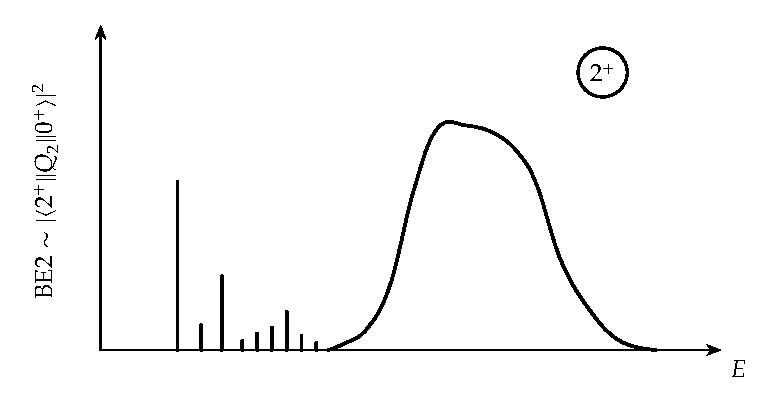
\includegraphics[width=0.75\linewidth]{pictures/1_6}
\par\end{centering}
\centering{}\caption{\label{fig:1_6}原子核中$2^{+}$能谱的示意图。纵坐标给出离散能级的$BE2$值以及共振区中的$BE2$强度密度。这些量表征向基态跃迁的概率。单位是任意的。}
\end{figure}

因此，低激发$2^{+}$态具有集体性质，即由许多粒子协同贡献，且常常被解释为表面四极振动。\ref{fig:1_7}给出了偶偶核中最低$2^{+}$态的能量$E_{2^{+}}$。可以观察到显著的壳效应（见第
2 章）。基于无旋流假设的液滴模型 {[}式 (1.19)、(1.30) 与 (1.34){]} 仅能给出平均趋势，其绝对值相差约
5 倍。

在实验上发现，第一$2^{+}$态的$BE2$值与其能量$E_{2^{+}_{1}}=\hbar\Omega_{2}$之间存在强烈的关联
\cite{Gr62}：
\begin{equation}
E_{2^{+}_{1}}B(E2,2^{+}\rightarrow0^{+})\simeq(25\pm8)\frac{Z^{2}}{A}\,[\text{MeV}\cdot e^{2}\cdot\text{fm}^{4}].\label{eq:1.40}
\end{equation}
这一经验关系在整个核素图的所有原子核中均成立。式 (1.39) 表现出相同的能量依赖性，但其对质量数$A$的依赖关系有所不同。低激发$2^{+}$态中显著的壳效应表明，它们不可能仅仅是纯粹的四极表面振荡，并且还存在具有这种集体振动性质的其他状态。由式
(1.22)、(1.21) 和 (1.35) 可见，四极表面振动在$\alpha$的线性阶下可表示为：
\begin{equation}
|2\mu)=B^{\dagger}_{2\mu}|0\rangle\propto\hat{\alpha}_{2\mu}|0\rangle\propto\hat{Q}_{2\mu}|0\rangle.\label{eq:1.41}
\end{equation}
因此，任意态$|\nu\rangle$与四极表面振动态的重叠正比于其$BE2$值：
\begin{equation}
|\langle\nu|2\mu\rangle|^{2}\propto|\langle\nu|\hat{Q}_{2\mu}|0\rangle|^{2}\propto B(E2,\nu\rightarrow0),\label{eq:1.42}
\end{equation}
而该态能被解释为这种振动的概率，由其耗尽求和规则的百分比给出：
\begin{equation}
S^{0}_{2\mu}=\sum_{\nu\neq0}|\langle\nu|\hat{Q}_{2\mu}|0\rangle|^{2}.\label{eq:1.43}
\end{equation}
只有当某个态在很大程度上耗尽了此求和规则时，将其称为四极表面振动才有明确的物理意义。

\begin{figure}[H]
\begin{centering}
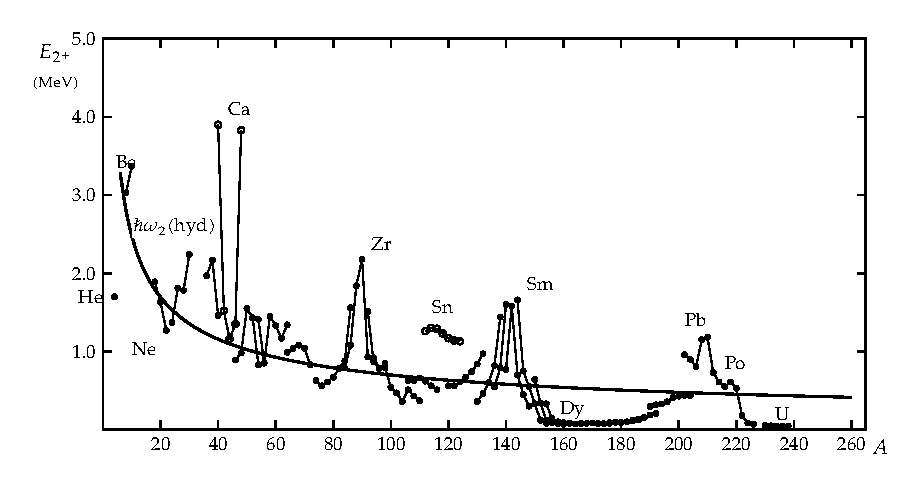
\includegraphics[width=0.85\linewidth]{pictures/1_7}
\par\end{centering}
\centering{}\caption{\label{fig:1_7}偶偶核中第一$2^{+}$态的能量。中子或质子为闭壳的核用空心圆圈标记（引自 \cite{NN65}）。}
\end{figure}

在 8.7 节中，我们将详细讨论求和规则及其计算方法。显而易见，在我们当前研究的模型中，态$\hat{Q}_{\lambda\mu}|0\rangle$是系统的本征态，因此该态完全耗尽了求和规则，因为所有其他态都与它正交。

在实验上发现，低激发$2^{+}$态通常仅耗尽求和规则的约 $10\%\sim20\%$。其主要部分被连续谱中的共振态所耗尽 {[}参见\ref{fig:1_6}{]}，即所谓的巨共振（giant
resonances）。

实验上已经观测到了具有不同自旋$I$的巨共振。最著名的便是巨偶极共振（$1^{-}$），三十多年来已广为人知，其能量位于（参见\ref{fig:1_8}，更详细讨论见第
13 章）：
\begin{equation}
\Omega^{\text{GR}}_{1}\simeq77\cdot A^{-1/3+-1/6}\,[\text{MeV}].\label{eq:1.44}
\end{equation}
正如我们将在第 8 章和第 13 章中看到的，它对应于中子球与质子球彼此相对的相对振动，无法在当前的简单模型中加以描述。

在近十年中，人们观测到了更多的巨共振。最重要的例子是同位旋标量巨四极共振。它所处的能量约为（参见\ref{fig:1_8}）：
\begin{equation}
\Omega^{\text{GR}}_{2^{+}}\simeq62\cdot A^{-1/3}\,[\text{MeV}],\label{eq:1.45}
\end{equation}
并且在多数情形下耗尽了$S_{2^{+}}$求和规则的大部分。

因此，将此共振解释为迄今所讨论的四极表面振动模似乎更为合理。然而，目前这种形式的液滴模型无法给出正确的质量数$A$依赖性。由式 (1.19)、(1.30)
和 (1.34) 可得
\[
\Omega_{2}\propto A^{-1/2},
\]
这与实验值 (1.45) 并不一致。在第 13 章中我们将看到，出现该偏差的原因在于：势能系数$C_{\lambda}$对应于液滴的总结合能
{[}(1.31)、(1.34){]}。然而，这一总结合能是内秉动能与势能之和。在式 (1.34) 中忽略了内秉动能（至少对小形变而言）对形变的依赖性。这可以简单理解为核子长平均自由程与不确定性原理的共同效应：不确定性原理指出，在椭球形状中，核子沿短轴方向的动量高于沿长轴方向的动量。然而，椭球形的动量分布比球形动量分布产生更大的动能。由于所有粒子均受到影响，这是一种体积效应，通常压倒了式
(1.34) 中给出的表面依赖性。在第 13 章中，我们将对这一点展开详细讨论。

\begin{figure}[H]
\begin{centering}
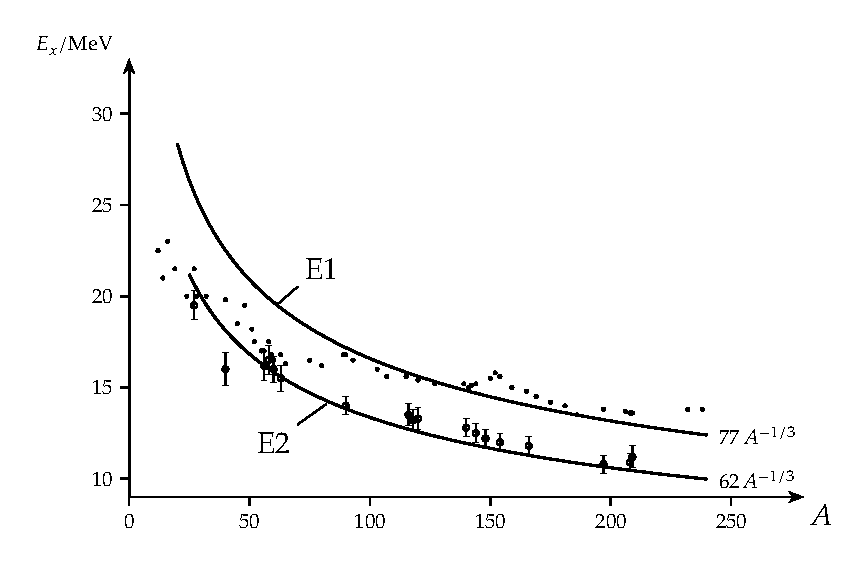
\includegraphics[width=0.75\linewidth]{pictures/1_8}
\par\end{centering}
\centering{}\caption{\label{fig:1_8}巨偶极共振与同位旋标量巨四极共振能量随质量数的变化关系 \cite{Wa73}。}
\end{figure}

尽管存在这些不足，但迄今为止所介绍的玻色子模型多年来仍得到了广泛应用，并在解释核谱的许多特征方面被证明相当成功 \cite{EG70}。其原因在于：许多低激发核态具有相当强的集体性质，可以很好地近似表示为玻色子。参数$B_{\lambda}$和$C_{\lambda}$在液滴模型中或许未能得到很好的给出，但正如我们将在第
8 章和第 9 章中所展示的，存在基于费米子的微观理论能够对$B_{\lambda}$和$C_{\lambda}$进行更为可靠的计算；因此，我们更应当将$B_{\lambda}$和$C_{\lambda}$视作开放的待定可调参数，而非由液滴模型所唯一决定。

微观理论还将表明，简谐近似 (1.17) 仅在极小振动的极限下具有非常粗略的有效性。对于具有较大振幅的集体运动，人们必须考虑非简谐项，例如
\[
\alpha^{4},\,\alpha^{2}\cdot\dot{\alpha}^{2},\,\dot{\alpha}^{4},\,\dots
\]
同样地，相应的参数既可以通过拟合实验来确定，也可以由微观多体理论计算得出（参见第 9 章）。

\section{形变的转动和振动\label{sec:=005F62=0053D8=007684=008F6C=0052A8=00548C=00632F=0052A8}\label{sec:1.5_=008F6C=0052A8=005E26}}

\subsection{Bohr Hamilton量\label{subsec:Bohr-Hamilton=0091CF}}

纯液滴模型仅在球形表面时具有稳定平衡。正如我们稍后将看到的（第 2.8 节），量子力学效应——即壳效应——可能导致集体 Hamilton
量中的势能$V(\boldsymbol{\alpha})$在有限非零值$\boldsymbol{\alpha}=\boldsymbol{\alpha}_{0}$处出现极小值。在此类情形下，原子核在基态即可具有稳定的形变。

在这种情况下，原子核可以展现出转动运动，该转动在实验室参考系中可由含时的表面参数$\alpha_{\lambda\mu}$来描述。我们将这些转动称为集体转动。绕对称轴的这种转动是不可能的，因为在我们的变量$\alpha_{\lambda\mu}$中，无法将转动后的系统与原始系统区分开来。

在量子力学描述中，具有对称轴（例如$z$轴）的系统由角动量算符$J_{z}$的本征波函数所描述，绕该对称轴的任何转动仅产生一个相位因子。因此，转动系统具有与基态相同的波函数和相同的能量。

这并不意味着系统中不存在其他可被激发并沿平行于对称轴方向携带角动量的自由度（例如单粒子自由度）。然而，这样一种“转动”我们并不称之为集体转动。

由于在几乎所有原子核中，四极自由度都起着根本性的作用，我们在下文中将把讨论局限于$\lambda=2$的情形。

假定原子核具有稳定的基态形变，最好将其变换到由质量分布主轴所定义的体固参考系中（如 1.3 节所讨论）。

完成该变换后，我们拥有五个动力学变量$\Omega$、$\beta$、$\gamma$\footnote{遗憾的是，Euler 角集合$\Omega=(\alpha,\beta,\gamma)$中也包含了字母$\beta$和$\gamma$。然而，我们不想改变这一通用命名习惯
\cite{Ed57}，因此尽可能采用缩写记号$\Omega$。}，用以代替原先的五个变量$\alpha_{2\mu}\,(\mu=-2,-1,0,+1,+2)$。我们再次从 Hamilton 量
(1.17) 出发，其中仅势能项发生改变，它现在的形式为：
\begin{equation}
V(\beta,\gamma)=\frac{1}{2}C_{20}(a_{20}(\beta,\gamma)-a^{0}_{20})^{2}+C_{22}(a_{22}(\beta,\gamma)-a^{0}_{22})^{2}.\label{eq:1.46}
\end{equation}
这对应于形变极小值$\beta_{0},\gamma_{0}$邻域内的二次近似。其物理图像是：原子核在其基态下具有这一形变，而激发态则是围绕此平衡形变的转动与小振动。

势能面的微观计算表明，对于某些特定的原子核，势能$V$在有限值$\beta_{0}\simeq0.2\sim0.3$以及$\gamma_{0}=0$处具有非常明显的极小值。因此，这些轴对称形状是最重要的情形，我们讨论的大部分内容都将针对它们展开。

下一步是将式 (1.17) 中的动能项变换到体固参考系。应用式 (1.11)，我们必须对变量$a_{20}$、$a_{22}$和$\Omega$对时间求导。由于该推导过程相当繁琐，且本章的目的并非包罗万象，我们仅给出所谓的
Bohr Hamilton 量 \cite{Bo52} 的结果（有关推导细节，参见例如 \cite[第 I 卷第 5 章]{EG70}）：
\begin{equation}
T=T_{\text{rot}}+\frac{1}{2}B_{2}(\dot{\beta}^{2}+\beta^{2}\dot{\gamma}^{2}),\label{eq:1.47}
\end{equation}
其中
\begin{equation}
T_{\text{rot}}=\frac{1}{2}\sum^{3}_{\kappa=1}\mathcal{J}_{\kappa}\omega^{2}_{\kappa},
\end{equation}
这里$\omega_{\kappa}$为绕体固$\kappa$轴的转动角速度，而$\mathcal{J}_{\kappa}$是由下式给出的$\beta$和$\gamma$的函数：
\begin{equation}
\mathcal{J}_{\kappa}=4B_{2}\beta^{2}\sin^{2}\left(\gamma-\frac{2\mathrm{\pi}}{3}\kappa\right),\quad\kappa=1,2,3.\label{eq:1.48}
\end{equation}
在我们固定形变$\beta,\gamma$的情形下，$T_{\text{rot}}$即为转动惯量为$\mathcal{J}_{\kappa}$的转子的动能。一旦我们允许$\beta$和$\gamma$发生变化，转动和振动自由度就会通过转动惯量对形变的依赖性耦合在一起。在这种情况下，我们不再拥有一个纯粹的转子。事实上我们看到，在$\beta_{0}=0$的情况下，该系统可以变换回具有谐振子谱的简谐振子
(1.17)。

然而，即使在具有较大刚度参数$C$和有限$\beta_{0}$的强形变情形下（此时常数近似$\beta=\beta_{0}$是相当好的近似），$\mathcal{J}_{\kappa}$也并不是刚体转子的转动惯量。利用式
(1.30)，我们由式 (1.48) 得到所谓的无旋流转动惯量：
\[
\mathcal{J}^{\text{irr}}_{\kappa}=\frac{3}{2\mathrm{\pi}}mAR^{2}_{0}\beta^{2}\sin^{2}\left(\gamma-\frac{2\mathrm{\pi}}{3}\kappa\right),\quad\kappa=1,2,3.
\]
它与具有相同形变的刚体转动惯量
\begin{equation}
\mathcal{J}^{\text{rig}}_{\kappa}=\frac{2}{5}mAR^{2}_{0}\left(1-\sqrt{\frac{5}{4\mathrm{\pi}}}\beta\cos\left(\gamma-\frac{2\mathrm{\pi}}{3}\kappa\right)\right)\label{eq:1.49}
\end{equation}
在以下几个方面存在显著差异：
\begin{enumerate}
\item 在$\gamma$依赖性方面（\ref{fig:1_9}），$\mathcal{J}^{\text{irr}}$在绕对称轴时严格为零。
\item $\mathcal{J}^{\text{irr}}$对形变具有强烈的依赖性（$\sim\beta^{2}$），而$\mathcal{J}^{\text{rig}}$随$\beta$的变化要弱得多（其主要部分是刚体球的转动惯量）。
\item 实验测得的转动惯量$\mathcal{J}^{\text{exp}}$可由转动带第一$2^{+}$态的能量求得 {[}参见式 (1.64){]}。即有$\mathcal{J}^{\text{exp}}=3/E_{2^{+}}$$[\text{MeV}^{-1}]$。结合经验规则
(1.40) 以及关于$BE2$值的公式 (1.74)，我们得到形变参数$\beta$与转动惯量之间的关联：
\begin{align}
\mathcal{J}^{\text{exp}} & =\frac{27}{80\mathrm{\pi}^{2}r^{4}_{0}}\frac{A^{4/3}\cdot\beta^{2}\cdot Z^{2}e^{2}}{E_{2^{+}}\cdot BE2}\approx\frac{27(1.2)^{4}\cdot\beta^{2}A^{7/3}}{80\mathrm{\pi}^{2}\cdot25}\nonumber \\
 & \approx\frac{\beta^{2}A^{7/3}}{400}\,[\text{MeV}^{-1}].\label{eq:1.50}
\end{align}
\end{enumerate}
在强形变核（$\beta\sim0.2\sim0.4$）的情形下，$\mathcal{J}^{\text{irr}}$通常比实验值小
2 到 3 倍。另一方面，$\mathcal{J}^{\text{rig}}$的值又比实验值大约 2 倍：
\begin{equation}
\mathcal{J}^{\text{irr}}<\mathcal{J}^{\text{exp}}<\mathcal{J}^{\text{rig}}.\label{eq:1.51}
\end{equation}
这表明原子核内部的流动结构绝非无旋流。另一方面，它也并非刚体转子。

接下来的步骤是对经典 Hamilton 量 (1.47) 进行量子化。众所周知，在一般情况下，经典 Hamilton 量的量子化并不存在唯一的法则
\cite{Me61}。这种不确定性源自不可对易算符排序的自由度\footnote{有关量子化问题的讨论与文献列表见 \cite{MD73}。}。通常人们采用
Pauli 法则 \cite{Pa33}，即在曲线坐标系中计算 Laplace 算符。若经典动能具有如下形式：
\begin{equation}
T=\frac{1}{2}\sum_{ij}g_{ij}(\boldsymbol{\xi})\dot{\xi}_{i}\dot{\xi}_{j},\label{eq:1.52}
\end{equation}

\begin{figure}[H]
\begin{centering}
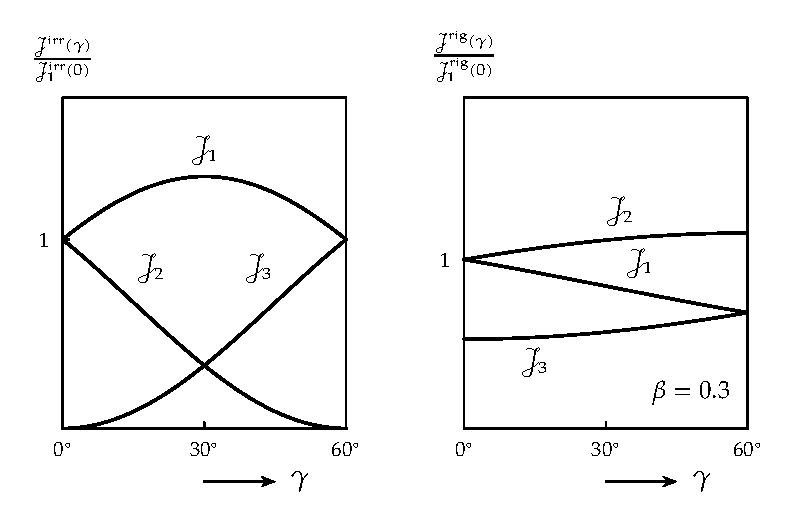
\includegraphics[width=0.75\linewidth]{pictures/1_9}
\par\end{centering}
\centering{}\caption{\label{fig:1_9}在固定的$\beta$值下，无旋流转动惯量（$\mathcal{J}^{\text{irr}}_{\kappa}$）与刚体转动惯量（$\mathcal{J}^{\text{rig}}_{\kappa}$）对$\gamma$的依赖关系。}
\end{figure}

则相应的量子化形式为\footnote{为了看清 Hamilton 量 (1.53) 是厄米的，必须计入体积元$\sqrt{g}\,\mathrm{d}\xi_{1}\dots\mathrm{d}\xi_{f}$。}：
\begin{equation}
\hat{H}_{\text{kin}}=-\frac{\hbar^{2}}{2}\sum_{ij}g^{-1/2}\frac{\partial}{\partial\xi_{i}}g^{1/2}(g^{-1})_{ij}\frac{\partial}{\partial\xi_{j}},\label{eq:1.53}
\end{equation}
其中$g$为矩阵$g_{ij}$的行列式，而$g^{-1}$为其逆矩阵。

将此法则应用于 Bohr Hamilton 量 (1.46) 和 (1.47)，我们得到：
\begin{align}
\hat{H}_{\text{coll}} & =-\frac{\hbar^{2}}{2B_{2}}\left[\beta^{-4}\frac{\partial}{\partial\beta}\left(\beta^{4}\frac{\partial}{\partial\beta}\right)+\frac{1}{\beta^{2}\sin3\gamma}\frac{\partial}{\partial\gamma}\left(\sin3\gamma\frac{\partial}{\partial\gamma}\right)\right]\nonumber \\
 & \quad+\hat{T}_{\text{rot}}+V(\beta,\gamma),\label{eq:1.54}
\end{align}
其中转动能为
\begin{equation}
\hat{T}_{\text{rot}}=\frac{\hat{I}^{2}_{1}}{2\mathcal{J}_{1}}+\frac{\hat{I}^{2}_{2}}{2\mathcal{J}_{2}}+\frac{\hat{I}^{2}_{3}}{2\mathcal{J}_{3}}.\label{eq:1.55}
\end{equation}
算符$\hat{I}_{\kappa}$为用 Euler 角表示的总角动量$\hat{\boldsymbol{I}}$在体固坐标轴上的投影（细节参见附录
A）。\ref{fig:1_10}展示了总角动量及其分量$\hat{I}_{z}=M$与$\hat{I}_{3}=K$。算符$\hat{\boldsymbol{I}}^{2}$、$\hat{I}_{z}$、$\hat{I}_{3}$的共同本征函数由下式给出：
\begin{equation}
|IMK\rangle=\sqrt{\frac{2I+1}{8\mathrm{\pi}^{2}}}D^{I*}_{MK}(\Omega).\label{eq:1.56}
\end{equation}
由于$H_{\text{coll}}$、$\hat{\boldsymbol{I}}^{2}$与$\hat{I}_{z}$彼此对易，集体
Hamilton 量的本征函数具有一般形式：
\[
|\Psi^{I}_{M}\rangle=\sum_{K}g_{K}(\beta,\gamma)|IMK\rangle.
\]

\begin{figure}[H]
\begin{centering}
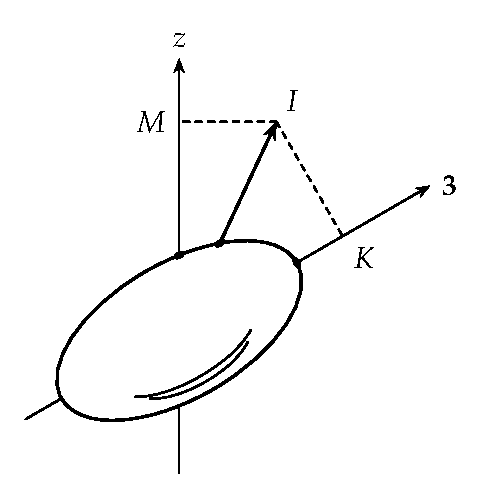
\includegraphics[width=0.75\linewidth]{pictures/1_10}
\par\end{centering}
\centering{}\caption{\label{fig:1_10}总角动量$I$与其在实验室$z$轴上的投影$M$以及在体固 3 轴上的投影$K$之间的关系。}
\end{figure}

三轴转子具有特定的离散对称性。$\hat{H}_{\text{coll}}$在点群$D_{2}$变换下保持不变 \cite{Bo52}。因此，可以根据该群的不可约表示对本征态进行分类，并由此推导出发射谱的若干性质
\cite{Da68}。

一个例子是绕 1 轴转动$180^{\circ}$的操作：
\begin{equation}
\mathscr{R}_{1}=\mathrm{e}^{\mathrm{i}\mathrm{\pi}\hat{I}_{1}},\label{eq:1.57}
\end{equation}
这等价于对 2, 3 平面的反射与宇称变换的复合。它与$\hat{H}_{\text{coll}}$对易，我们要求本征函数具有本征值$+1$\footnote{正如我们将在式 (11.123) 中看到的，系统的微观内秉波函数是该操作本征值为$+1$的本征态（亦参见 \cite{Bo76b}）。}：
\begin{equation}
\mathscr{R}_{1}|\Psi^{I}_{M}\rangle=|\Psi^{I}_{M}\rangle.\label{eq:1.58}
\end{equation}
利用附录 A 中的关系式 (A.24)，我们发现这仅在满足下述条件时才可能成立：
\begin{equation}
g_{K}(\beta,\gamma)=(-)^{I}g_{-K}(\beta,\gamma).\label{eq:1.59}
\end{equation}
同理，若我们要求对如下转动的对称性：
\begin{equation}
\mathscr{R}_{2}=\mathrm{e}^{\mathrm{i}\mathrm{\pi}\hat{I}_{2}},\label{eq:1.60}
\end{equation}
则得到
\begin{equation}
g_{K}(\beta,\gamma)=(-)^{I+K}g_{-K}(\beta,\gamma).\label{eq:1.61}
\end{equation}


\subsection{轴对称情形\label{subsec:=008F74=005BF9=0079F0=0060C5=005F62}}

Hamilton 量$\hat{H}_{\text{coll}}$ (1.54) 仍然非常一般。我们在此将限制于势能面在轴对称形变$\beta=\beta_{0}$和$\gamma=0$处具有非常显著极小值的情形。我们预期核表面会出现转动和小振动。将式
(1.55) 中的$T_{\text{rot}}-\hat{I}^{2}_{3}/2\mathcal{J}_{3}$围绕点$\beta=\beta_{0},\gamma=0$展开，在零阶近似下我们得到转动惯量为$\mathcal{J}_{0}=\mathcal{J}_{1}(\beta_{0},0)=\mathcal{J}_{2}(\beta_{0},0)$的轴对称转子的
Hamilton 量：
\begin{equation}
T^{\prime}_{\text{rot}}=\frac{\hat{\boldsymbol{I}}^{2}-\hat{I}^{2}_{3}}{2\mathcal{J}_{0}}.\label{eq:1.62}
\end{equation}
一阶项正比于偏离量$(\beta-\beta_{0})$与$\gamma$。它们使转动与振动自由度相混合（转动-振动耦合项），在此处予以略去。在$H_{\text{coll}}$中仍然耦合转动与振动的唯一项是$\hat{I}^{2}_{3}/2\mathcal{J}_{3}$。由于$\mathcal{J}_{3}$在$\gamma=0$时为零，该项不能被展开。然而（如同$T^{\prime}_{\text{rot}}$），它与$\hat{I}_{3}$对易，因此$K$是一个好量子数。

我们现在必须区分两种情形：

\paragraph*{(i) $K=0$ 带（$I_{3}=0$）。}

在这种情况下，转动与振动运动解耦。波函数具有如下形式：
\begin{equation}
|\Psi^{I}_{M0}\rangle=g_{0}(\beta,\gamma)|IM0\rangle.\label{eq:1.63}
\end{equation}
它们是 Hamilton 量 (1.54) 转动部分的本征函数。$\mathscr{R}_{1}$对称性 (1.59) 要求自旋序为$I=0,2,4,\dots$。对$H_{\text{coll}}$振动部分的详细研究
\cite[第 I 卷第 6 章]{EG70} 表明，在变量$a_{20}$和$a_{22}$ (1.13)
下处理更为简便。在第一步中，人们略去势能$V(a_{20},a_{22})$中将这两个自由度耦合起来的交叉项。在此情形下，沿坐标$a_{20}$的运动（通常称为$\beta$振动）与沿坐标$a_{22}$的运动（通常称为$\gamma$振动）解耦。绕
3 轴的轴对称性在$\beta$振动（量子数为$n_{\beta}$）下得以保持，但在$\gamma$振动（量子数为$n_{\gamma}$）下被破坏。\ref{fig:1_11}定性地展示了这两种运动形式。

叠加在每个振动态$(n_{\beta},n_{\gamma})$之上的是一个转动带。其能谱由下式给出（参见 \cite[第 I 卷第 6 章]{EG70}）：
\begin{equation}
E_{n_{\beta}n_{\gamma}}(I)=E_{n_{\beta}n_{\gamma}}(0)+\frac{\hbar^{2}}{2\mathcal{J}_{0}}I(I+1),\label{eq:1.64}
\end{equation}
其带头能量为：
\begin{equation}
E_{n_{\beta}n_{\gamma}}(0)=\hbar\omega_{\beta}\left(n_{\beta}+\frac{1}{2}\right)+\hbar\omega_{\gamma}(2n_{\gamma}+1),\quad n_{\beta}=0,1,2,\dots,\quad n_{\gamma}=0,1,2,\dots,\label{eq:1.65}
\end{equation}
其中$\omega_{\beta}$和$\omega_{\gamma}$分别为$\beta$振动和$\gamma$振动的频率：
\[
\omega_{\beta}=(C_{20}/B_{2})^{1/2},\quad\omega_{\gamma}=(C_{22}/B_{2})^{1/2}.
\]
事实上，在许多偶偶核中都观测到了这样的能带，特别是基态带（$n_{\beta}=n_{\gamma}=0$）与“$\beta$带”（$n_{\beta}=1,n_{\gamma}=0$）。然而，正如我们前面所讨论的，流体动力学模型给出的常数$\mathcal{J}_{0}$以及$\omega_{\beta},\omega_{\gamma}$与实验数据并不相符。

\paragraph*{(ii) $K\protect\neq0$ 带。}

结合$\mathscr{R}_{1}$对称性 {[}式 (1.58){]}，我们看到此时波函数具有如下形式：
\begin{equation}
|\Psi^{I}_{MK}\rangle=g_{K}(\beta,\gamma)\frac{1}{\sqrt{2}}\left(|IMK\rangle+(-)^{I}|IM-K\rangle\right).\label{eq:1.66}
\end{equation}
$\mathscr{R}_{1}$与$\mathscr{R}_{2}$对称性（式 (1.59) 和 (1.61)）给出了选择定则：$K$必须为偶数。因此，这样的$K\neq0$带具有自旋序列$I=|K|,|K|+1,|K|+2,\dots$。沿$a_{20}$的运动（$\beta$振动）同样可以与其余部分分离。然而，项$\hat{I}^{2}_{3}/2\mathcal{J}_{3}=K^{2}/16B_{2}a^{2}_{22}$将$\gamma$振动与绕
3 轴的转动耦合在一起。如果我们认识到$\gamma$振动可以表示为三轴核绕 3 轴以相反$K$值进行的两次转动的叠加，就很容易理解这一事实
\cite[第 656 页]{BM75}。

由此得到如下能谱 \cite[第 I 卷第 6 章]{EG70}：
\begin{equation}
E_{K,n_{\beta},n_{\gamma}}(I)=E_{K,n_{\beta},n_{\gamma}}(0)+\frac{\hbar^{2}}{2\mathcal{J}_{0}}(I(I+1)-K^{2}),\label{eq:1.67}
\end{equation}

\begin{figure}[H]
\begin{centering}
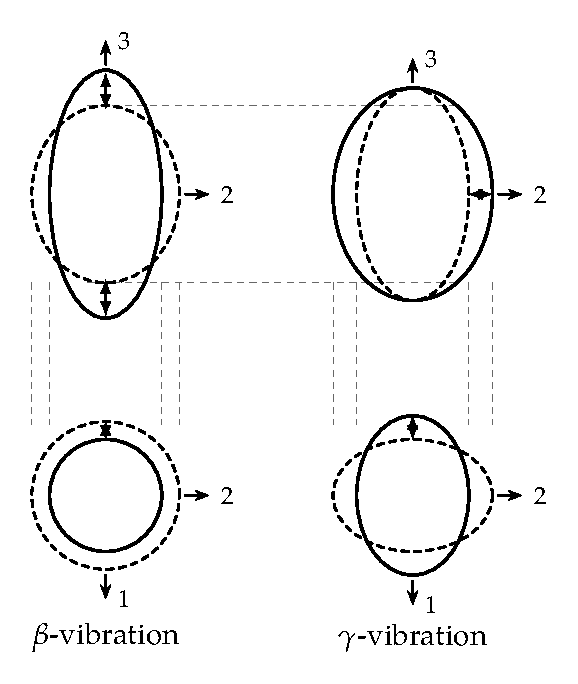
\includegraphics[width=0.75\linewidth]{pictures/1_11}
\par\end{centering}
\centering{}\caption{\label{fig:1_11}通过沿 (1, 3) 与 (1, 2) 平面剖切示意性表示的$\beta$振动与$\gamma$振动。}
\end{figure}

其带头能量为：
\begin{equation}
E_{K,n_{\beta},n_{\gamma}}(0)=\hbar\omega_{\beta}\left(n_{\beta}+\frac{1}{2}\right)+\hbar\omega_{\gamma}\left(2n_{\gamma}+1+\frac{|K|}{2}\right).\label{eq:1.68}
\end{equation}
事实上，这类能带也已被观测到，特别是在许多形变核中具有量子数$K=2,n_{\beta}=0,n_{\gamma}=0$的所谓“$\gamma$带”。虽然该$\gamma$带的振动量子数为$n_{\gamma}=0$，但在此情形下绝不能套用无振动的经典图像。因为经典无振动图像对应于$\gamma=0$，从而意味着$\mathcal{J}_{3}=0$，这将禁戒$K\neq0$的转动。正是量子力学在$\gamma$方向上的零点振动才使得这种激发成为可能。

\ref{fig:1_12}给出了形变核与球形核中集体（$\lambda=2$）激发的定性结构。

球形核具有简谐谱。在形变核中，我们观察到建立在基态、$\beta$振动态（$K=0,n_{\beta}=1,n_{\gamma}=0$）以及$\gamma$振动态（$K=2,n_{\beta}=0,n_{\gamma}=0$）之上的若干转动带。然而，这些纯粹的情形在自然界中并未严格实现。事实上，我们已经在球形核中观察到了双玻色子三重态（$0^{+},2^{+},4^{+}$）的劈裂，并在形变核中观察到了对$I(I+1)$规律的偏离。在两个极限之间还存在着大范围的过渡核。从一种同位素到另一种同位素，人们有时可以观察到从振动谱到转动谱的平滑过渡（例如在
Os 区核中 \cite{SDG76}）。这在\ref{fig:1_12}中用虚线示意给出。

\begin{figure}[H]
\begin{centering}
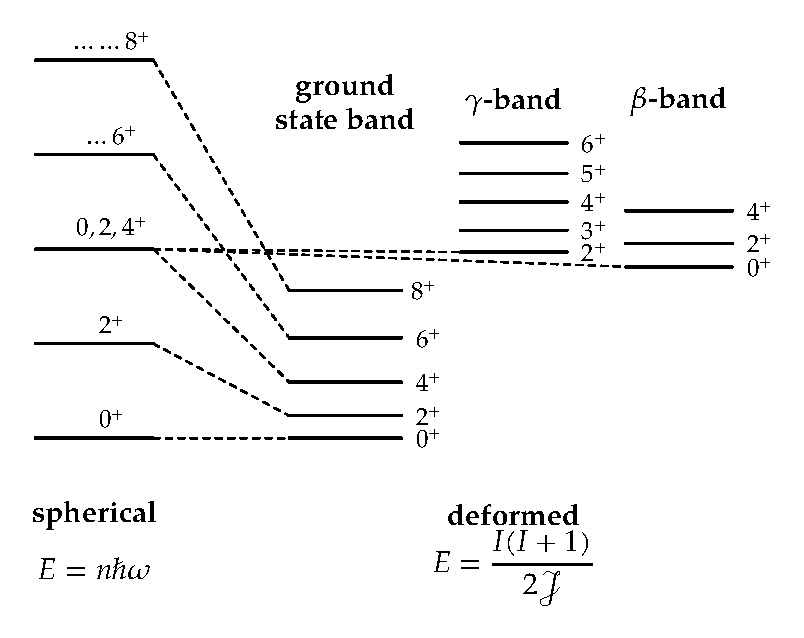
\includegraphics[width=0.75\linewidth]{pictures/1_12}
\par\end{centering}
\centering{}\caption{\label{fig:1_12}球形核与形变核能级方案的示意图（引自 \cite{SDG76}）。}
\end{figure}

为了从理论上描述对$I(I+1)$规律的偏离，人们考虑了$\hat{H}_{\text{coll}}$中的转动-振动耦合项，这些项是通过将$\mathcal{J}_{\kappa}$按偏离量$(\beta-\beta_{0})$和$\gamma$的幂次展开而得到的
\cite{FG62,FG64,FGS65,FGS66,ABP68}。这种转动-振动相互作用引起能带转动惯量的变化，对应于原子核形状在转动影响下的形变拉伸（stretching
effect）。然而，在这一能区内还存在着原子核截然不同的其他激发，例如双准粒子态和配对振动（参见第 8 章），它们对转动带的影响要强得多，而这些在带有表面振动的简单液滴模型中并未加以考虑。

在结束本节之前，我们简要讨论如何计算电磁极矩和跃迁概率。在式 (1.35) 和 (1.36) 中，我们利用坐标$\alpha_{\lambda\mu}$定义了电多极矩和磁偶极矩算符。它们显然是在实验室坐标系中写出的。在形变核中，在内秉参考系中计算极矩通常极为方便。为了得到实验室参考系中的极矩——即实验测得的值——必须应用球张量的变换关系
(1.11)：
\begin{equation}
\hat{Q}^{\text{intr}}_{\lambda\mu}=\sum_{\mu^{\prime}}D^{\lambda}_{\mu^{\prime}\mu}\hat{Q}^{\text{lab}}_{\lambda\mu^{\prime}}.\label{eq:1.69}
\end{equation}
由于$Q^{\text{intr}}$不依赖于 Euler 角，根据 \cite[式 4.6.2 和 5.4.1]{Ed57}，我们得到在基底$|IMK\rangle$下的约化矩阵元：
\begin{equation}
\langle I_{1}K_{1}||\hat{Q}^{\text{lab}}_{\lambda}||I_{2}K_{2}\rangle=\sum_{\mu^{\prime}}Q^{\text{intr}}_{\lambda\mu^{\prime}}(-)^{I_{1}-K_{1}}((2I_{1}+1)(2I_{2}+1))^{1/2}\begin{pmatrix}I_{1} & \lambda & I_{2}\\
-K_{1} & \mu^{\prime} & K_{2}
\end{pmatrix}.\label{eq:1.70}
\end{equation}
我们现在限制于纯$K$带，且仅计算带内$E2$跃迁（$n_{\gamma_{1}}=n_{\gamma_{2}},n_{\beta_{1}}=n_{\beta_{2}}$）。对于约化矩阵元，我们求得：
\begin{equation}
\langle n_{\beta}n_{\gamma}I_{1}K||\hat{Q}^{\text{lab}}_{2}||n_{\beta}n_{\gamma}I_{2}K\rangle=\sqrt{\frac{5}{16\mathrm{\pi}}}Q_{0}(n_{\beta},n_{\gamma})\sqrt{(2I_{1}+1)(2I_{2}+1)}(-)^{I_{1}-K}\begin{pmatrix}I_{1} & 2 & I_{2}\\
-K & 0 & K
\end{pmatrix},\label{eq:1.71}
\end{equation}
其中$Q_{0}(n_{\beta},n_{\gamma})$为该能带的内秉四极矩。在固定$\beta$值且$\gamma=0$的基态带中，由式
(1.13) 和 (1.35) 可得：
\begin{equation}
Q_{0}=\sqrt{\frac{16\mathrm{\pi}}{5}}\frac{3}{4\mathrm{\pi}}Ze\cdot R^{2}_{0}\cdot\beta.\label{eq:1.72}
\end{equation}
由式 (B.73) 与 (1.71)，我们例如可以求得转动带中所谓的跨跃（stretched）$BE2$值：
\begin{equation}
B(E2,I+2\rightarrow I)=Q^{2}_{0}\frac{5}{16\mathrm{\pi}}|C^{I+2\,2\,I}_{K\,0\,K}|^{2},\label{eq:1.73}
\end{equation}
对于$K=0$带，该式给出：
\begin{equation}
B(E2,I+2\rightarrow I)=Q^{2}_{0}\frac{5}{16\mathrm{\pi}}\frac{3}{2}\frac{(I+1)(I+2)}{(2I+3)(2I+5)}.\label{eq:1.74}
\end{equation}
对于光谱学四极矩$Q=\sqrt{16\mathrm{\pi}/5}\langle IIK|\hat{Q}^{\text{lab}}_{20}|IIK\rangle$
{[}式 (B.32){]}，我们得到：
\begin{equation}
Q=Q_{0}\frac{3K^{2}-I(I+1)}{(2I+3)(I+1)}.\label{eq:1.75}
\end{equation}
商值$Q:Q_{0}$即为态$M=I$中$D^{2}_{00}=P_{2}(\cos\beta)$的期望值。这意味着人们无法直接测量内秉四极矩$Q_{0}$，而只能测得在转动运动上平均的值。事实上，$Q_{0}$并非一个严格的物理可观测量。它的定义依赖于随原子核共同运动的体固坐标系的引入，具有模型依赖的性质。对于带头通常有$I=K$。这意味着具有$I=0$的基态的光谱学四极矩$Q$为零，我们只能对激发态获得关于$Q_{0}$的信息（例如通过
Coulomb 激发中的重取向效应（reorientation effect）\cite{BE68}，它给出了$Q_{0}$的符号与绝对值）。确定$Q_{0}$绝对值的另一种方法是测量带内跃迁的$B(E2)$值
(1.73)。近年直至高自旋态的测量表明 \cite{WCL76,HJE78}，在许多形变核中，即使能谱显示出对$I(I+1)$特性的偏离，$Q_{0}$的值在这些带内仍保持相当稳定。这提示我们，这些偏离并非由形变的改变（拉伸效应）所主导。

\subsection{非对称转子\label{subsec:=00975E=005BF9=0079F0=008F6C=005B50}}

迄今所讨论的转动-振动相互作用模型均建立在对称转子的基础之上。Davydov 等人利用纯三轴转子的图像进行了进一步尝试，以解释对$I(I+1)$规律的偏离以及许多核中低激发的第二个$2^{+}$态
\cite{DF58,DR59,Da59,Da65b}。作为第一步，他们不考虑振动激发，而仅对转动能 (1.55) 进行对角化。利用转动惯量
(1.48)，该算符正比于$\beta^{-2}$，并且可以针对任意$\gamma$值进行对角化。常数因子随后可通过拟合第一$2^{+}$态来调节。利用对称性$\mathscr{R}_{1}$与$\mathscr{R}_{2}$（式
(1.59) 和 (1.61)），波函数具有如下形式：
\begin{equation}
|\Psi^{I}_{M}\rangle=\sum_{K=0,2,\dots}g_{K}\left\{ |IMK\rangle+(-)^{I}|IM-K\rangle\right\} .\label{eq:1.76}
\end{equation}
\ref{fig:1_13}给出了相应的能量本征值。在$\gamma=0^{\circ}$和$\gamma=60^{\circ}$时，人们得到标准的$I(I+1)$能谱。即使在较强的三轴形变下，对该形式的偏离也微乎其微。然而，额外的$2^{+},3^{+},4^{+}$能级在能量上下降。具有低激发的第二个$2^{+}$态是该结构的显著特征。虽然利用这样一个模型可以相当合理地复现某些元素周期表区域（例如
Os 同位素）的实验数据，但人们仍对它提出了强烈的异议：
\begin{enumerate}
\item 它无法描述$\beta$振动。若要描述$\beta$振动，必须引入额外的振动自由度 \cite{DC60}。
\item 能够确立稳定$\gamma$形变的显著能面极小值迄今尚未被发现。对此类过渡核的微观计算通常显示沿$\gamma$方向只有非常浅的平坦能谷
\cite{KB68,ASS69,GPA72,GG78}\footnote{Wilets 和 Jean \cite{WJ56} 提出了一个完全对$\gamma$软（$\gamma$-soft）的模型，即在式
(1.46) 中设$C_{22}=0$。}。
\end{enumerate}
近年来，稳定的$\gamma$形变重新引起了人们的浓厚兴趣，因为：
\begin{enumerate}
\item 奇$A$过渡核中的实验数据可以通过单粒子耦合于非对称转子的模型得到极好的复现（参见第 5 章以及 \cite{MSD74,Me75,TF75}）。
\item 针对极高自旋态的理论计算表明（参见 1.7 节及 \cite{ALL76}），原子核在特定自旋区域内可能变为三轴形变。
\end{enumerate}
通过假定极大三轴度（$\gamma=30^{\circ}$），人们可以对三轴核的能级结构给出一个粗略的估计。在这种情形下，$\mathcal{J}_{2}=\mathcal{J}_{3}=\frac{1}{4}\mathcal{J}_{1}=\frac{1}{4}\mathcal{J}_{0}$（$\mathcal{J}_{0}$为在$\gamma=0$处的转动惯量），并且（在动能中）我们具有关于
1 轴的对称性。角动量$\boldsymbol{I}$在此轴上的投影$\alpha$是一个好量子数，由此求得：
\begin{equation}
E_{\alpha}(I)=\frac{3\hbar^{2}}{8\mathcal{J}_{0}}(4I(I+1)-3\alpha^{2}).\label{eq:1.77}
\end{equation}

\begin{figure}[H]
\begin{centering}
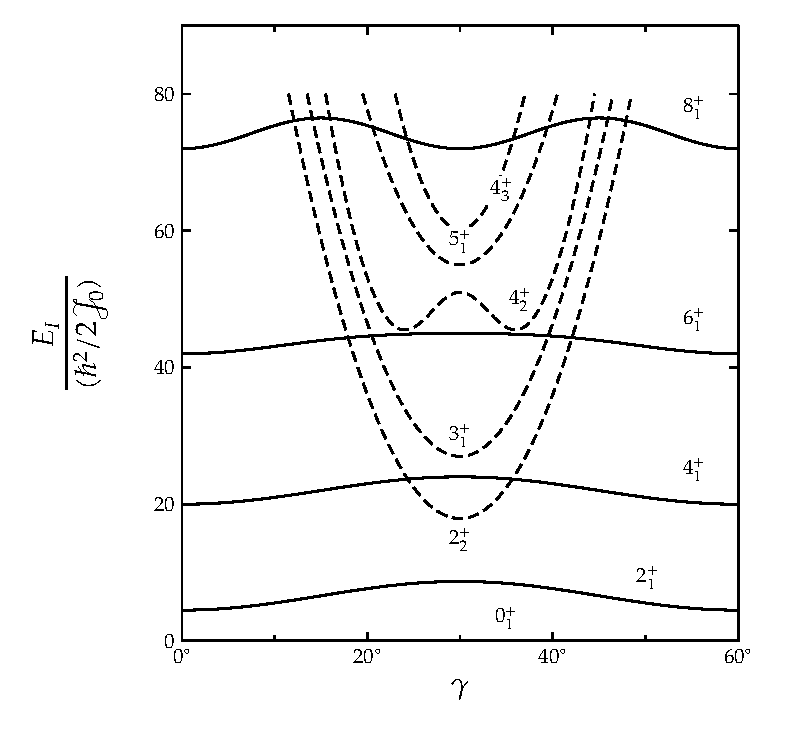
\includegraphics[width=0.75\linewidth]{pictures/1_13}
\par\end{centering}
\centering{}\caption{\label{fig:1_13}具有流体动力学转动惯量的形变非对称转子的能量本征值（引自 \cite{Me75}）。}
\end{figure}

$\mathscr{R}_{1}$与$\mathscr{R}_{2}$对称性要求$I$和$\alpha$均为偶数。对于每个$I$，具有最低能量的能级（即所谓的“yrast”能级）对应于$\alpha=I$。能量次低的能带对应于$\alpha=I-2$，继而是$\alpha=I-4$，依此类推。因此，我们得到了一系列由“摆动”（wobbling）量子数$n=I-\alpha$所表征的能带
\cite{BM75}。可以计算出，具有相同$n$的态之间由很大的$E2$跃迁概率所联接。我们由式 (1.77) 得到它们的能谱：
\begin{equation}
E_{n}(I)=\frac{3\hbar^{2}}{8\mathcal{J}_{0}}(I(I+4)+3n(2I-n)).\label{eq:1.78}
\end{equation}
然而必须牢记，能谱的结构（\ref{fig:1_13}）极度敏感地依赖于转动惯量对$\gamma$的依赖关系。在该图中采用的是流体动力学值。若采用刚体值，能谱的面貌无疑将大为改观。

\section{核裂变\label{sec:=006838=0088C2=0053D8}}

到目前为止，我们在液滴模型中仅研究了围绕平衡形状的小振动。在核裂变被发现后不久，人们便尝试运用核液滴的概念来理解这一现象 \cite{MF39,Fr39,BW39}。

事实上，一个均匀带电的经典液滴，仅在 Coulomb 能不超过某一临界值时才对裂变是稳定的（且保持球形）。Coulomb 排斥倾向于使液滴发生形变，从而使粒子平均而言相距更远。相反，表面能正比于液滴的表面积，倾向于使其保持球形。因此，这两种效应（各自的绝对量级均达数百个
MeV）之间的微妙平衡过程，依据经典计算决定了是否会发生裂变。当然，对于涉及大形变的裂变过程，人们必须超越前几节所讨论的简谐近似 \cite{BW39}。

描述裂变过程的第一步 \cite{HW53} 是选取一组适当的形变参数，我们记作$\boldsymbol{\alpha}$。它必须足够普遍，以能够描述可能出现的所有形变。例如，Cohen
和 Swiatecki \cite{CS62,CS63} 在计算如下形式的对称形状时，考虑了多达 18 阶的多极展开：
\begin{equation}
R=R_{0}\left(1+\sum^{18}_{l=1}\alpha_{l}P_{l}(\cos\theta)\right).\label{eq:1.79}
\end{equation}
这使得人们能够描述非常普遍的几何形状。另一方面，如果人们定性地了解液滴在裂变过程中的演化行为，就会希望引入尽可能少的参数。由于人们还希望描述已分离的碎片，因此参数集
(1.79) 显然不是最合适的。为了对裂变过程进行现实的描述，至少需要三个参数 \cite{NS65,Ni72}：
\begin{enumerate}
\item 参数$c$：在裂变过程开始时在某种意义上描述长半轴的长度，并平滑过渡为已分离碎片之间的间距（伸长坐标，elongation coordinate）；
\item 参数$h$：表征正在形成的碎片之间颈部的厚度（颈部坐标，neck coordinate）；
\item 非对称参数$\alpha_{s}$：度量分离碎片质量分布偏离对称性的程度（在非对称裂变情形下）（碎裂坐标，fragmentation
coordinate）。
\end{enumerate}
\ref{fig:1_14}给出了这种参数化方案的一个实例 \cite{BDJ72}。

\begin{figure}[H]
\begin{centering}
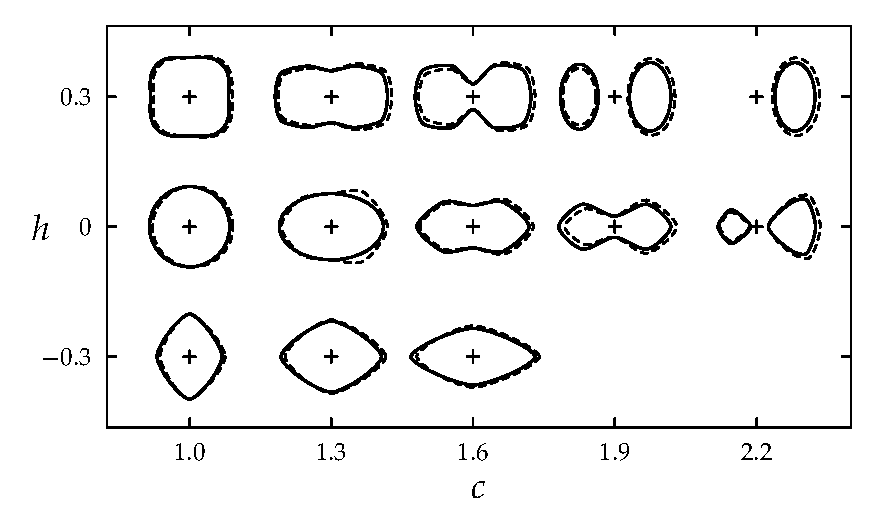
\includegraphics[width=0.85\linewidth]{pictures/1_14}
\par\end{centering}
\centering{}\caption{\label{fig:1_14}在一组适宜的参数化方案$\{c,h\}$下的若干原子核形状。实线表示对称形状；虚线具有非零的非对称参数$\alpha_{s}$（引自
\cite{BDJ72}）。}
\end{figure}

下一步必须计算参数$\boldsymbol{\alpha}$下的 Hamilton 量。首先是势能项$V(\boldsymbol{\alpha})$。人们通常以相应球体的表面能\footnote{如我们前面所讨论的，势能可以具有对应于内秉动能的体积依赖性。然而，对于裂变过程所涉及的大形变，动力学效应对$V(\boldsymbol{\alpha})$可能产生重要影响：通常假定自发裂变过程非常缓慢，以至于核子有充裕的时间调整其动量分布，从而在每个形变下使总能量最小。该动量分布自然是球对称的动量分布。（有关此点的更详细讨论见第
13 章。）}为单位来度量它，得到：
\begin{equation}
V(\boldsymbol{\alpha})=(B_{s}(\boldsymbol{\alpha})-1)+2x(B_{C}(\boldsymbol{\alpha})-1),\label{eq:1.80}
\end{equation}
其中$B_{s}$和$B_{C}$分别为表面能 {[}以$E_{s}(0)$为单位{]} 与 Coulomb 能 {[}以$E_{C}(0)=\frac{3}{5}(eZ)^{2}/R_{0}$为单位{]}。它们的计算类似于式
(1.32) 和 (1.33)。然而，此时人们不能再假定小形变，而必须显式完成各重积分。$B_{s}$和$B_{C}$仅取决于几何形状。表征特定原子核的唯一参数是所谓的可裂变度参数（fissibility
parameter）$x$。我们求得：
\begin{equation}
x=\frac{E_{C}(0)}{2E_{s}(0)}=\frac{Z^{2}/A}{(Z^{2}/A)_{\text{crit}}},\label{eq:1.81}
\end{equation}
其中
\begin{equation}
\left(\frac{Z^{2}}{A}\right)_{\text{crit}}=\frac{40\mathrm{\pi}}{3}\frac{r^{3}_{0}\sigma}{e^{2}}\approx50.\label{eq:1.82}
\end{equation}
Cohen 与 Swiatecki 的计算 \cite{CS62,CS63} 表明，使原子核发生形变最容易的途径是四极形变，且核液滴总体上要么保持球形，要么发生裂变。因此，在零形变处，我们就可以依据势能面$V(\boldsymbol{\alpha})$在原点处沿四极方向的曲率是正还是负，来判定裂变是否发生。然而，这正是我们在考虑
Bohr Hamilton 量 {[}式 (1.17){]} 直至二次项时所已经计算过的。确实，我们看到刚度系数$C_{2}$ {[}式
(1.34){]} 由形变能的表面部分与 Coulomb 部分之差给出，且当满足下式时$C_{2}$开始变为负值 \cite{Wi64}：
\begin{equation}
\frac{Z^{2}}{A}=\left(\frac{Z^{2}}{A}\right)_{\text{crit}}\quad\text{或}\quad x=1.\label{eq:1.83}
\end{equation}
这意味着经典液滴在$Z^{2}/A\lesssim50$或$x<1$时保持稳定且呈球形。对于$x>1$，它立即发生裂变。这一结论可以通过向水银滴上不断增加电荷的实验得到验证。

对于$^{238}\text{U}$，质量公式 (1.4) 给出的 Coulomb 能约为$E_{C}(0)\approx830\,\text{MeV}$，表面能约为$E_{s}(0)\approx520\,\text{MeV}$；因此我们求得可裂变度参数为$x\simeq0.8$，这是该质量区（$230<A<240$）的典型数值。因此，经典液滴模型无法描述自发裂变。实验中观测到的自发裂变完全归因于量子力学的隧穿效应。

液滴的势能面 (1.80) 通常具有非常复杂的结构。对于$x<1$，我们预期存在一个对应于球体的极小值，而在大间距处存在对应于不同碎裂通道的出射能谷
\cite{NS65,Ni69,MN76}。

例如，若仅考虑对称裂变，针对两个参数$c$和$h$，我们得到如\ref{fig:1_15}所示的能量面。可以看到，它形成了一个定义明确的鞍点（saddle）。在鞍点外侧，形变能急剧下降。

\begin{figure}[H]
\begin{centering}
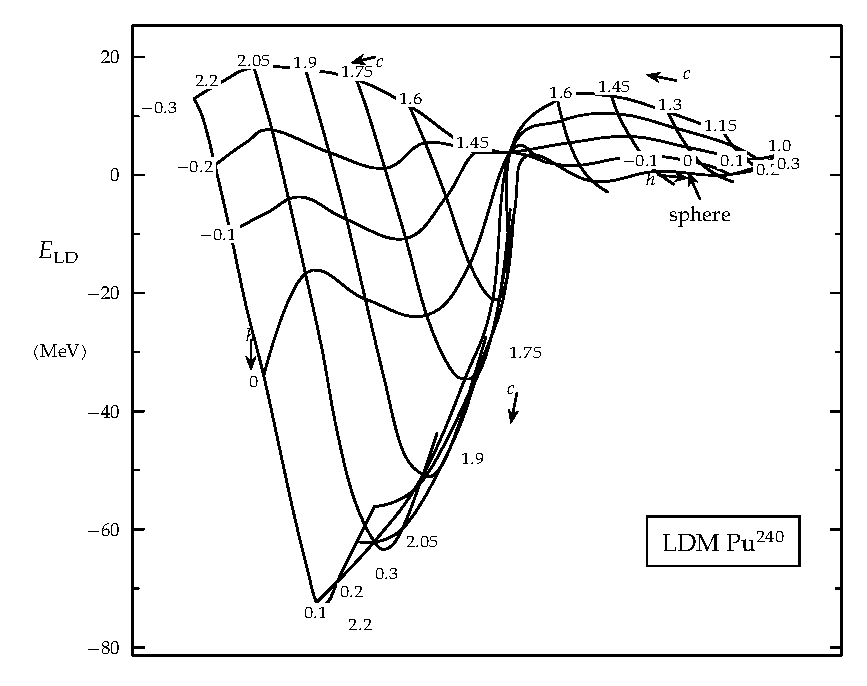
\includegraphics[width=0.85\linewidth]{pictures/1_15}
\par\end{centering}
\centering{}\caption{\label{fig:1_15}$^{240}\text{Pu}$ 液滴模型能量面的透视图。$h$ 描述伸长自由度，$c$
描述颈缩自由度（引自 \cite{BDJ72}）。}
\end{figure}

Cohen 和 Swiatecki \cite{CS63} 利用拟设 (1.79) 计算了许多$x$值下的鞍点形状，其中一部分展示在\ref{fig:1_16}中。

这些鞍点形状的物理含义是：对于给定的$x$，粗略地说，如果使液滴的伸长量比鞍点稍微再大一点，它就不可避免地滑向裂变；反之，若使其伸长量稍微缩短一点，它就会回弹回球形形状。沿着最陡下降线越过鞍点，裂变谷的“谷底”定义了一条一维路径。沿着这条路径的弧长通常称为裂变坐标$s$。\ref{fig:1_17}示意性地展示了沿该坐标的势能分布。

\begin{figure}[H]
\begin{centering}
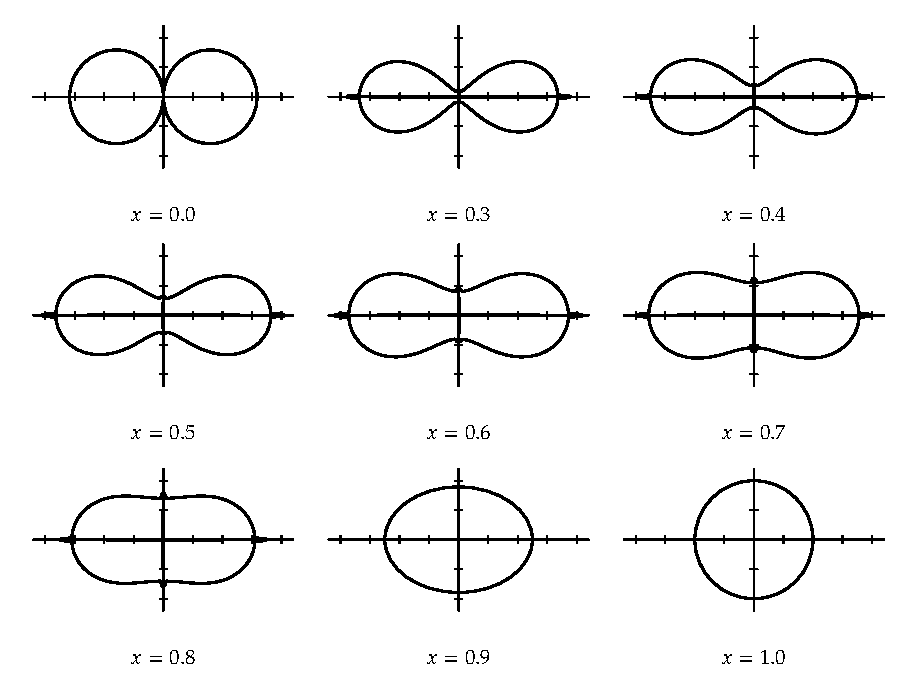
\includegraphics[width=0.85\linewidth]{pictures/1_16}
\par\end{centering}
\centering{}\caption{\label{fig:1_16}可裂变度参数$x$取不同值时的鞍点形状（引自 \cite{CS63}）。}
\end{figure}

裂变势垒高度$E_{B}$通常只有几个 MeV，例如 $5\sim7\,\text{MeV}$。（这应当与数千 MeV 的总结合能相对比）。在相距很远的外侧区域，曲线的下降斜率纯粹源于两个小液滴之间的
Coulomb 排斥，因而对于大$Z$核下降得十分陡峭。

\begin{figure}[H]
\begin{centering}
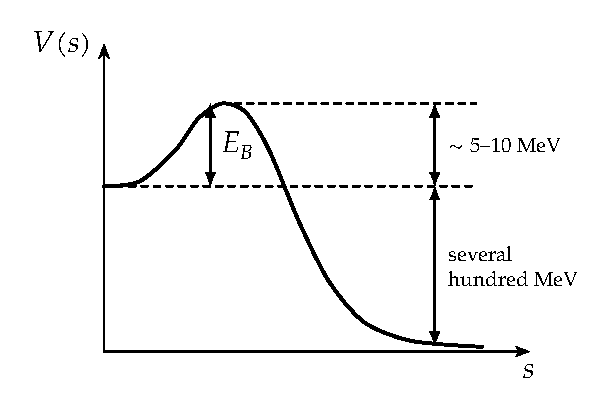
\includegraphics[width=0.75\linewidth]{pictures/1_17}
\par\end{centering}
\centering{}\caption{\label{fig:1_17}液滴裂变势垒的示意图。}
\end{figure}

在裂变的动力学描述中，下一步将是计算动能（即质量参数，它们无疑依赖于形变 \cite{HD71,Gr71}）。既然流体动力学模型在处理小振动时未能给出令人满意的质量参数，我们自然无法指望它在此处能有良好表现。我们将在
12.3.7 节中看到通常如何计算这些物理量。

最终的步骤将是合理的量子化以及对所得 Schrödinger 方程的求解。详细讨论这些问题远远超出了本章的范围。我们在此仅指出，通常由一维势垒穿透的
WKB 公式来计算自发裂变的寿命 \cite{Wi64}。该公式的核心输入要素正是势能$V(s)$的形状，如\ref{fig:1_17}所示。

遗憾的是，液滴模型无论如何都无法定量地描述核裂变，其主要缺陷之一在于：液滴总是裂变为两个质量相等的碎片，而实验中原子核却极频繁地裂变为质量不等的两块碎片（非对称裂变）。裂变势垒是一个由两个巨大数字相减所得的微小数值，这一事实表明核裂变是一个极其微妙的过程，我们很容易理解，单粒子运动中的量子效应（如壳效应，见
2.9 节）会对它产生决定性的深刻影响。

\section{转动液滴的稳定性\label{sec:=008F6C=0052A8=006DB2=006EF4=007684=007A33=005B9A=006027}}

我们在 1.5 节中已经看到，在液滴围绕球形表面的振动中存在着类似于转动的运动。然而，为了将转动从振动中解耦出来，我们要求存在稳定的有限形变，而这只能由量子力学的壳效应来解释。事实上，实验中观测到的转动谱充分证实了这一假定的合理性。

重离子碰撞实验使得向原子核注入极大的角动量（高达 $80\sim100\,\hbar$）成为可能。在如此高的激发下，人们预期微观量子效应不再起支配作用，于是人们自然要追问：具有如此高旋转角速度的经典液滴将如何表现？

因此，在本节中我们仅关注一个纯粹的经典问题：一个具有清晰表面、带有电荷且具有一定表面能的不可压缩液滴，在绕空间固定轴转动时将具有怎样的物理行为。我们对表面振动不感兴趣，而是寻求该系统的稳定平衡形状。

我们再次需要对液滴内部的流动结构作出假定，在此我们将假定为刚体转动；即转动惯量由下式给出：
\begin{equation}
\mathcal{J}=\mathcal{J}^{\text{rig}}=\int_{V}r^{2}_{\perp}\rho_{0}\,\mathrm{d}^{3}\boldsymbol{r},\label{eq:1.84}
\end{equation}
其中$r_{\perp}$是体积元$\mathrm{d}^{3}\boldsymbol{r}$距转动轴的垂直距离。正如我们将在
3.4 节中看到的，该假定非常合理，因为人们预期在高角动量极限下原子核的转动惯量将趋近于刚体转动惯量值。

这一问题与天体物理中著名的自引力不可压缩均匀旋转质量体问题非常相似。在天体问题中，吸引力是万有引力，它与 Coulomb 力具有完全相同的数学结构（但符号相反），且表面力被忽略不计。从
Newton 开始，这一问题就被许多著名数学家广泛研究（历史评述见 \cite[第 1 章]{Ch69}）。

所得结果之一是：没有表面张力的自引力液滴在转动角速度$\omega\rightarrow0$时呈球形。当$\omega>0$时，它首先呈现严格的以转动轴为对称轴的扁椭球形状（Maclaurin
形状）。随着$\omega$的增大，它变得越来越扁，直到某一临界角速度$\omega_{I}$。对于大于$\omega_{I}$的$\omega$值，出现了一种新型的稳定形状\footnote{这对应于一个二级相变 \cite{BR76}。}——三轴椭球（Jacobi
形状）——此时液滴绕其最短的主轴转动。该点$\omega_{I}$称为分叉点（bifurcation point），因为当$\omega>\omega_{I}$时，Maclaurin
形状虽然仍是定态极值解，但在某些自由度上已不再是能量极小值 \cite{Ro67}。人们称之为长期不稳定（secularly unstable）。然而，在没有摩擦力的均匀转动系统（陀螺系统）中，它们仍能表现出稳定的运动（普通稳定性，ordinary
stability）\cite{Ly58}。沿着 Jacobi 形状向更高的$\omega$值追踪，将到达进一步的分叉点，演化出新的平衡形状，直至最终液滴破裂瓦解。

Cohen、Plasil 与 Swiatecki \cite{CPS74} 研究了转动核液滴的稳定性问题。他们寻找能量面的驻点解：
\begin{align}
E(\boldsymbol{\alpha}) & =E_{s}(\boldsymbol{\alpha})+E_{C}(\boldsymbol{\alpha})+E_{R}(\boldsymbol{\alpha})\nonumber \\
 & =E_{s}(0)(B_{s}(\boldsymbol{\alpha})+2x\cdot B_{C}(\boldsymbol{\alpha})+yB_{R}(\boldsymbol{\alpha})).\label{eq:1.85}
\end{align}
除了表面能（$E_{s}$）与 Coulomb 能（$E_{C}$）之外 {[}参见式 (1.32) 等{]}，我们现在还计入了在给定角动量$I$下的转动能：
\begin{equation}
E_{R}(\boldsymbol{\alpha})=\frac{\hbar^{2}I^{2}}{2\mathcal{J}(\boldsymbol{\alpha})}=yE_{s}(0)B_{R}(\boldsymbol{\alpha}).\label{eq:1.86}
\end{equation}
零形变下的转动惯量由式 (1.84) 给出：$\mathcal{J}(0)=\frac{2}{5}MR^{2}_{0}$。除了度量
Coulomb 能与表面能相对比例的可裂变度参数$x$之外，现在还出现了新的旋转参数：
\begin{equation}
y=\frac{E_{R}(0)}{E_{s}(0)}=\frac{5}{16\mathrm{\pi}}\frac{\hbar^{2}I^{2}}{\sigma mr^{4}_{0}}\frac{1}{A^{7/3}}\approx2I^{2}A^{-7/3},\label{eq:1.87}
\end{equation}
它度量了转动能与表面能的相对大小。参数$x$和$y$完全由原子核本身的内秉属性以及所感兴趣的角动量决定；其余的计算纯粹是几何学问题。

这些研究 \cite{CPS74} 的结论是：原子核的表现与自引力液滴极为相似。在低角动量（低$y$值）下，原子核呈现绕转动轴轴对称的扁平形状。它们被称为
Hiskes 形状，与严格的扁椭球（Maclaurin 形状）十分相似。它们在达到临界值$y_{I}$（对应于 Jacobi 点）之前保持稳定。$y_{I}$的数值依赖于$x$。对于极重核$x>0.81$，当$y>y_{I}$时系统直接发生裂变。对于其余的原子核，则演化出一种新型的稳定形状。这些形状被称为
Beringer-Knox 形状 \cite{BK61}，与 Jacobi 形状相似。在极高角动量下，这些形状绕垂直于原对称轴的轴变得近乎轴对称，并最终对裂变变得不稳定（$y_{II}$）。

上述计算涉及大量的形变参数。如果将形状限制为严格的三轴椭球，其半轴$a_{1},a_{2},a_{3}$可由两个参数$\beta$和$\gamma$所表征\footnote{我们此前在描述核表面的微小四极形变时已经使用了 Hill-Wheeler 坐标$\beta$与$\gamma$ {[}式 (1.13){]}。在此我们通过半轴将核表面定义为严格的椭球。这正是
Hill 和 Wheeler \cite{HW53} 的原始定义。它仅在小$\beta$值极限下才与式 (1.7) 一致。}：
\begin{equation}
a_{\kappa}=R_{0}\exp\left\{ \sqrt{\frac{5}{4\mathrm{\pi}}}\beta\cos\left(\gamma-\frac{2\mathrm{\pi}}{3}\kappa\right)\right\} \quad(\kappa=1,2,3).\label{eq:1.88}
\end{equation}
该定义保证了体积的守恒性。

\begin{figure}[H]
\begin{centering}
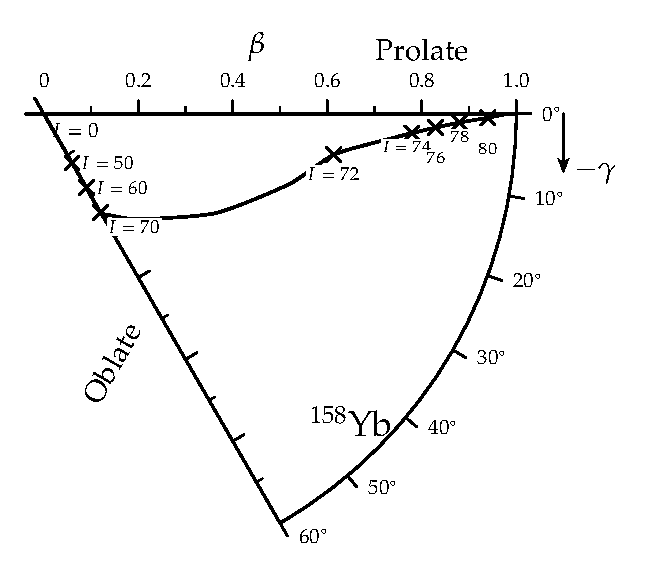
\includegraphics[width=0.75\linewidth]{pictures/1_18}
\par\end{centering}
\centering{}\caption{\label{fig:1_18}作为角动量$I$函数的转动液滴平衡形状（以$\beta$和$\gamma$表示）。由于 1
轴为转动轴，与通常三个轴完全等价的情形相反，此处需要负的$\gamma$值。核素$^{158}\text{Yb}$的参数值为$x=0.618$（引自
\cite{ALL76}）。}
\end{figure}

计算这些椭球的刚体转动惯量、表面能与 Coulomb 能\footnote{参见例如 \cite{Ca61,CM63}。}作为$\beta$和$\gamma$的函数相对较为简便，并可进而寻找对应于每个$I$值的能量面极小值。将这些稳定平衡形状连接起来，便在$\beta$-$\gamma$平面上得到一条轨迹，如\ref{fig:1_18}所示。

对于每个给定的$I$，我们都拥有一张能量曲面并研究其局域极小值。正如在$I=0$的情形下一样（1.6 节），除了极小值之外，还存在着一个带有鞍点的裂变能谷。由于离心力的作用，势垒高度随着角动量的增加而减小；当势垒彻底消失时，该形状族对裂变变得完全不稳定。作为一个例子，我们考虑原子核$^{127}\text{La}$
\cite{CPS74}。在零角动量$I=0$时，其液滴模型裂变势垒高达$40.0\,\text{MeV}$。其 Jacobi
点（$y_{I}$）对应于$I=67.8\,\hbar$。在此角动量下，其激发能达到$44.31\,\text{MeV}$ {[}$E_{s}(0)=49.5\,\text{MeV}${]}，而裂变势垒高度骤降至仅剩$7.8\,\text{MeV}$。

从这一考量中可以清晰地看出：任何原子核都无法承受超过某一极限角动量的旋转，否则它将对裂变发生失稳。在\ref{fig:1_19}中，展示了处于$\beta$稳定线
{[}由$N=A/2+0.2\cdot A^{2}/(200+A)$所近似{]} 上的原子核裂变势垒完全消失时的角动量$I_{II}$随质量数$A$的变化关系。轻核由于自身尺寸过小而无法承载过多的角动量单位；重核由于
Coulomb 能的排斥而稳定性降低；位于$A\simeq130$附近的原子核可以达到最高的旋转角动量（约$100\,\hbar$）。重离子碰撞实验
\cite{BES76} 的结果与液滴模型给出的这些极限值表现出良好的一致性。

\begin{figure}[H]
\begin{centering}
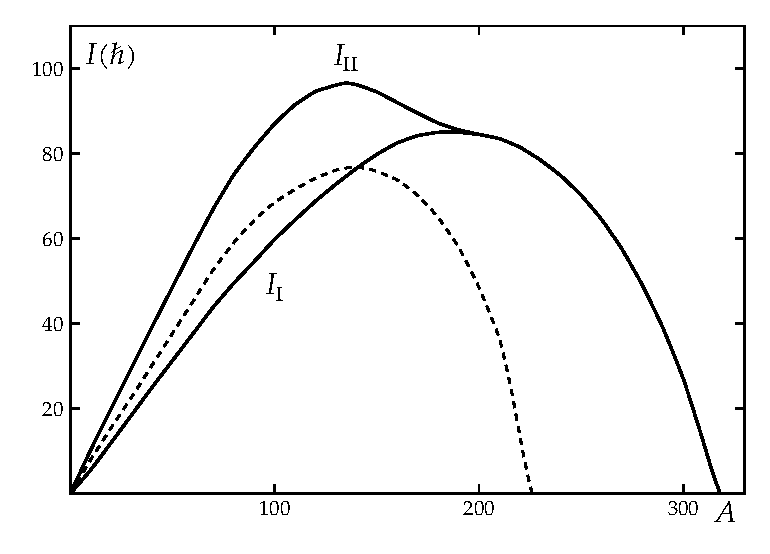
\includegraphics[width=0.75\linewidth]{pictures/1_19}
\par\end{centering}
\centering{}\caption{\label{fig:1_19}处于$\beta$稳定线上的质量数为$A$的原子核所能承受的最大角动量$I_{II}$以及临界角动量$I_{I}$（Jacobi
分叉点）。虚线对应于裂变势垒高度为$8\,\text{MeV}$的曲线，这一势垒高度保证了对裂变具有合理的寿命（引自 \cite{CPS74}）。}
\end{figure}

